\documentclass[preprint, 3p,
authoryear]{elsarticle} %review=doublespace preprint=single 5p=2 column
%%% Begin My package additions %%%%%%%%%%%%%%%%%%%

\usepackage[hyphens]{url}

  \journal{Nature Climate Change - initial submission: supplementary
information} % Sets Journal name

\usepackage{graphicx}
%%%%%%%%%%%%%%%% end my additions to header

\usepackage[T1]{fontenc}
\usepackage{lmodern}
\usepackage{amssymb,amsmath}
% TODO: Currently lineno needs to be loaded after amsmath because of conflict
% https://github.com/latex-lineno/lineno/issues/5
\usepackage{lineno} % add
\usepackage{ifxetex,ifluatex}
\usepackage{fixltx2e} % provides \textsubscript
% use upquote if available, for straight quotes in verbatim environments
\IfFileExists{upquote.sty}{\usepackage{upquote}}{}
\ifnum 0\ifxetex 1\fi\ifluatex 1\fi=0 % if pdftex
  \usepackage[utf8]{inputenc}
\else % if luatex or xelatex
  \usepackage{fontspec}
  \ifxetex
    \usepackage{xltxtra,xunicode}
  \fi
  \defaultfontfeatures{Mapping=tex-text,Scale=MatchLowercase}
  \newcommand{\euro}{€}
\fi
% use microtype if available
\IfFileExists{microtype.sty}{\usepackage{microtype}}{}
\usepackage[]{natbib}
\bibliographystyle{elsarticle-harv}

\ifxetex
  \usepackage[setpagesize=false, % page size defined by xetex
              unicode=false, % unicode breaks when used with xetex
              xetex]{hyperref}
\else
  \usepackage[unicode=true]{hyperref}
\fi
\hypersetup{breaklinks=true,
            bookmarks=true,
            pdfauthor={},
            pdftitle={APPENDIX to European Carbon Market Connectedness and Risk Contagion: A Study of Return and Volatility Dynamics Between Post-Phase II European Union Allowances (EUAs) and Financial Markets and their Potential for Portfolio Diversification},
            colorlinks=false,
            urlcolor=blue,
            linkcolor=magenta,
            pdfborder={0 0 0}}

\setcounter{secnumdepth}{5}
% Pandoc toggle for numbering sections (defaults to be off)


% tightlist command for lists without linebreak
\providecommand{\tightlist}{%
  \setlength{\itemsep}{0pt}\setlength{\parskip}{0pt}}




\usepackage{subcaption, graphicx, pdflscape, float} \graphicspath{ {./figures/} }



\begin{document}


\begin{frontmatter}

  \title{APPENDIX to European Carbon Market Connectedness and Risk
Contagion: A Study of Return and Volatility Dynamics Between Post-Phase
II European Union Allowances (EUAs) and Financial Markets and their
Potential for Portfolio Diversification}
      \cortext[cor1]{Corresponding author}
  
  \begin{abstract}
  
  \end{abstract}
  
 \end{frontmatter}

\newpage

\appendix

\begin{landscape}
\section{Static Return and Volatility Connectedness Matrix} \label{apdx:ConnMatrix}
  \begin{table}[!ht]
    \caption{Static Return and Volatility Connectedness Matrix (Jan 2013 - Jan 2025)}
    \label{table:staticfull}
      \resizebox{\columnwidth}{!}{
      \begin{tabular}{|l|l|l|l|l|l|l|l|l|l|l|l|} 
        \multicolumn{12}{@{}l}{\em(a) Carbon returns connectedness matrix}\\ \hline
      & CARBON & EUROSTOXX & BRENT OIL & COAL API & NATGAS & EURSOVER & EURCORP & SPXINDEX & COMEXENG & METALS & DSF (FROM) \\ \hline
       CARBON & 60.06 & 4.00 & 3.80 &   7.85 & 10.21 & 2.48 &   2.26 & 3.47 &   2.76    & 3.11 & \textbf{39.94} \\ \hline
       EUROSTOXX & 3.28 &   49.76 & 5.70 & 3.33 &   3.12 & 3.05 &   3.67 & 19.87 & 5.20 &   3.03 & 50.24 \\ \hline
       BRENTOIL & 3.49 &    6.00 &  57.40 & 5.44 &  3.61 &  2.68 &  2.34 &  7.27 &  8.29 &  3.49 &  42.60 \\ \hline
       COALAPI & 6.34 & 3.77 &  5.80 &  56.02 & 13.78 & 1.85 &  2.04 &  3.84 &  3.96 &  2.62 &  43.98 \\ \hline
       NATGAS & 9.93 &  3.03 &  3.88 &  13.58 & 58.73 & 1.80 &  1.76 &  2.48 &  2.56 &  2.24 &  41.27 \\ \hline
       EURSOVER & 2.03 &    2.98 &  2.68 &  1.67 &  1.68 &  48.35 & 31.93 & 2.28 &  2.05 &  4.36 &  51.65 \\ \hline
       EURCORP & 1.97 & 5.05 &  2.71 &  1.75 & 1.81 &   30.37 & 45.49 & 3.97 &  2.54 &  4.35 &  54.51 \\ \hline
       SPXINDEX & 2.42 &    17.95 & 6.82 &  3.35 &  2.03 &  2.30 &  2.73 &  53.51 & 6.40 &  2.50 &  46.49 \\ \hline
       COMEXENG & 2.48 &    5.08 &  7.44 &  3.49 &  2.40 &  2.16 &  2.37 &  6.59 &  53.07 & 14.91 & 46.93 \\ \hline
       METALS & 2.37 &  3.15 &  3.10 &  2.28 &  2.47 &  4.83 &  5.59 &  2.96 &  16.14 & 57.11 & 42.89 \\ \hline
       DST (TO) & \textbf{34.31} & 51.01 &  41.93 & 42.73 & 41.10 & 51.52 & 54.69 & 52.73 & 49.89 & 40.60 & 460.50 \\ \hline
       Inc.Own & 94.37 & 100.77 &   99.33 & 98.75 & 99.83 & 99.87 & 100.18 &    106.24 &    102.96 &    97.70 & \textbf{TCI} \\ \hline
       NS (NET) & \textbf{-5.63} & 0.77 &   -0.67 & -1.25 & -0.17 & -0.13 & 0.18 &  6.24 &  2.96 &  -2.30 & \textbf{46.05} \\ \hline
        \end{tabular}
        }
\bigskip\bigskip
         \resizebox{\columnwidth}{!}{
         \begin{tabular}{|l|l|l|l|l|l|l|l|l|l|l|l|} 
          \multicolumn{12}{@{}l}{\em(b) Carbon volatility connectedness matrix}\\ \hline
       & CARBON & EUROSTOXX & BRENTOIL & COALAPI & NATGAS & EURSOVER & EURCORP & SPXINDEX & COMEXENG & METALS & DSF (FROM) \\ \hline
       CARBON & 55.66 & 4.60 &  4.29 &  7.25 &  7.13 &  3.77 &  3.61 &  5.06 &  3.83 &  4.79 & \textbf{44.34} \\ \hline
       EUROSTOXX & 3.63 &   47.09 & 5.17 & 3.59 &   3.45 &  5.12 &  4.14 &  16.60 & 5.25 &  5.95 &  52.91 \\ \hline
       BRENTOIL & 4.20 &    6.54 &  52.55 & 4.93 &  3.59 &  3.85 &  4.54 &  6.49 &  7.10 &  6.20 &  47.45 \\ \hline
       COALAPI & 4.67 & 5.83 &  4.19 &  57.95 & 7.85 &  3.80 &  2.71 &  4.59 &  3.14 &  5.26 &  42.05 \\ \hline
       NATGAS & 4.51 &  4.64 &  3.43 &  8.36 &  59.40 & 3.52 &  3.79 &  4.82 &  3.56 &  3.96 &  40.60 \\ \hline
       EURSOVER & 2.17 &    6.27 &  3.30 &  2.43 &  1.86 &  44.69 & 25.39 & 5.60 & 3.86 &   4.44 &  55.31 \\ \hline
       EURCORP & 2.81 & 5.70 &  2.52 &  2.34 &  2.40 &  28.32 & 41.90 & 5.97 &  4.70 &  3.33 &  58.10 \\ \hline
       SPXINDEX & 3.29 &    15.44 & 5.03 &  3.08 &  1.71 &  4.71 &  3.98 &  53.15 & 4.44 &  5.17 &  46.85 \\ \hline
       COMEXENG & 2.62 &    7.96 &  4.69 &  3.94 &  4.00 &  5.32 &  5.39 &  6.71 &  49.30 & 10.07 & 50.70 \\ \hline
       METALS & 3.91 &  8.31 &  4.44 &  3.90 &  3.85 &  5.08 &  6.31 &  6.26 &  10.05 & 47.90 & 52.10 \\ \hline
       DST (TO) & \textbf{31.83} & 65.30 &  37.07 & 39.82 & 35.85 & 63.47 & 59.86 & 62.11 & 45.92 & 49.18 & 490.40 \\ \hline
       Inc.Own & 87.49 &    112.39 &    89.62 & 97.77 & 95.25 & 108.16 &    101.76 &    115.27 &    95.22   & 97.08 & \textbf{TCI} \\ \hline
       NS (NET) & \textbf{-12.51} & 12.39 & -10.38 &    -2.23 & -4.75 & 8.16 &  1.76 &  15.27 & -4.78 & -2.92 & \textbf{49.04} \\ \hline
        \end{tabular}
        }
\end{table}




\section{Dynamic Return and Volatility Net Directional Connectedness}  \label{apdx:NDC}
\begin{figure}[H]
  \caption{Dynamic Net Directional Connectedness (Jan 2013 – Jan 2025)}
  \label{fig:dynNDCfull}
    \centering
      \begin{subfigure}[a]{\textwidth}
        \caption{Dynamic return net directional connectedness}
        \label{fig:dynretNDCfull}
        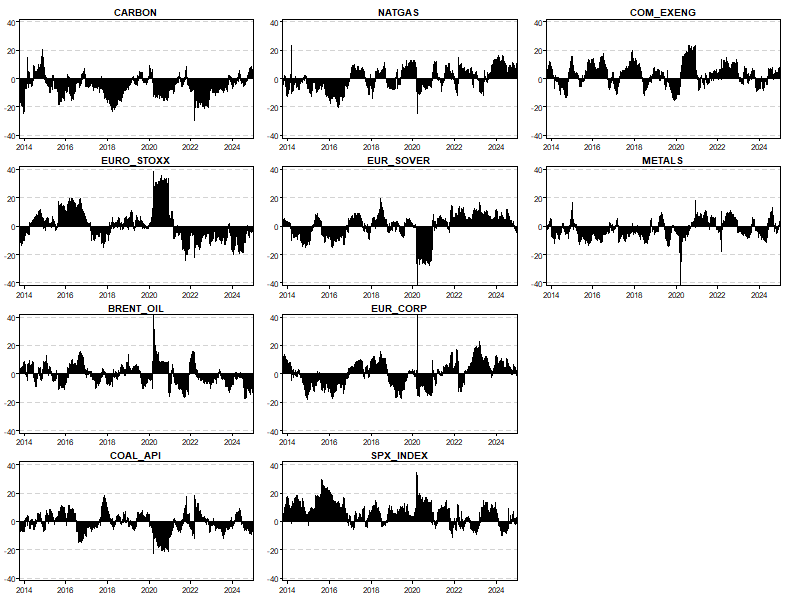
\includegraphics[width = 1.25\linewidth]{6aApdxB-DynRetNDCfull}
      \end{subfigure}
\end{figure}
\begin{figure}[H]
  \ContinuedFloat
  \centering
      \begin{subfigure}[b]{\textwidth}
        \caption{Dynamic volatility net directional connectedness}
        \label{fig:dynvolNDCfull}
        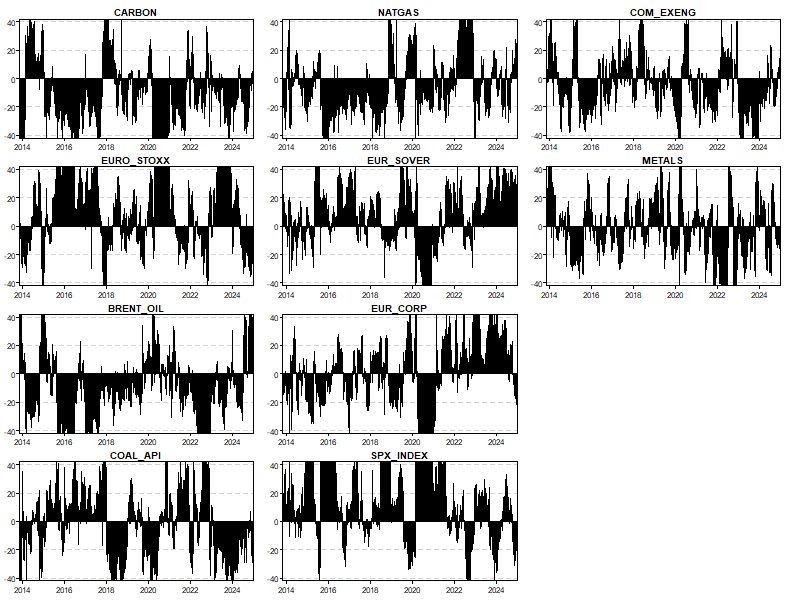
\includegraphics[width = 1.25\linewidth]{6bApdxB-DynVolNDCfull}
      \end{subfigure}
\end{figure}

\newpage

\section{Dynamic Return and Volatility Pairwise Connectedness Index} \label{apdx:PCI}
\begin{figure}[!ht]
  \caption{Dynamic Return and Volatility Pairwise Connectedness Index (Jan 2013 – Jan 2025)}
  \label{fig:dynPCIfull}
  \centering
  \begin{subfigure}[a]{\textwidth}
    \caption{Dynamic return PCI}
    \label{fig:dynretPCIfull}
    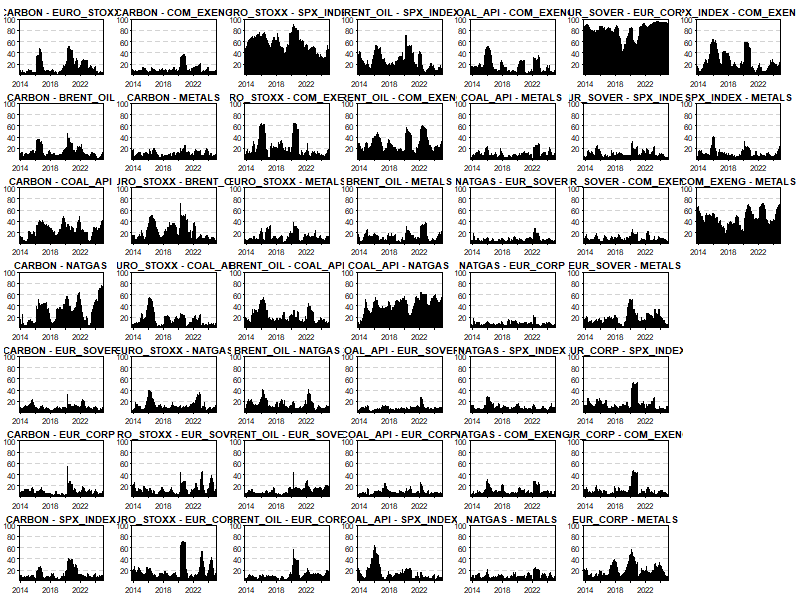
\includegraphics[width = 1.1\linewidth]{7aApdxC-DynRetPCIfull}
  \end{subfigure}
\end{figure}
\begin{figure}[!ht]
  \ContinuedFloat
  \centering
    \begin{subfigure}[b]{\textwidth}\ContinuedFloat
      \caption{Dynamic volatility PCI}
      \label{fig:dynvolPCIfull}
      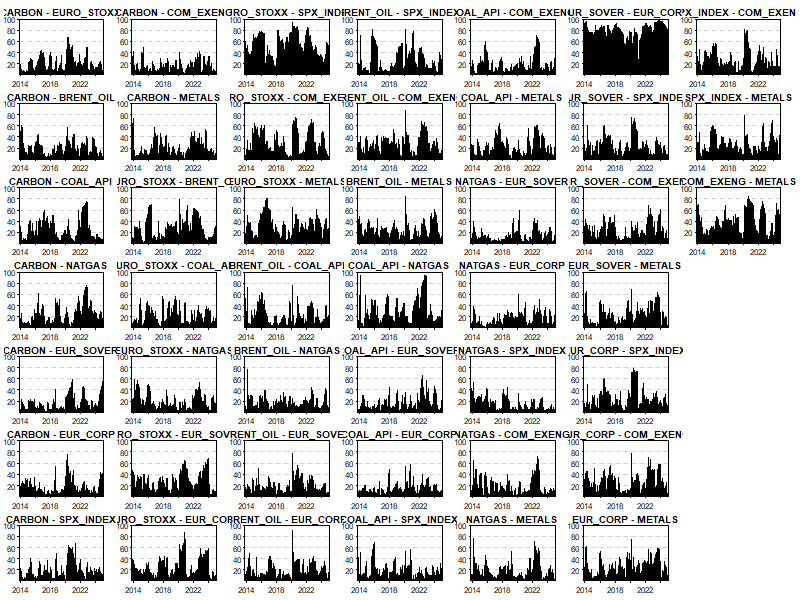
\includegraphics[width = 1.2\linewidth]{7bApdxC-DynVolPCIfull}
    \end{subfigure}
\end{figure}


\newpage

\section{Robustness Testing of Connectedness Model Parameters} \label{apdx:Robust}
\subsection{10-period forecast horizon and a rolling window of 180 observations}

\subsubsection{Static Return and Volatility Connectedness Matrix}

  \begin{table}[!ht]
    \caption{Static Return and Volatility Connectedness Matrix (Jan 2013 - Jan 2025)}
      \resizebox{\columnwidth}{!}{
      \begin{tabular}{|l|l|l|l|l|l|l|l|l|l|l|l|}
      \multicolumn{12}{@{}l}{\em(a) Carbon returns connectedness matrix}\\ \hline
        ~ & CARBON & EUROSTOXX & BRENTOIL & COALAPI & NATGAS & EURSOVER & EURCORP & SPXINDEX & COMEXENG & METALS & FROM \\ \hline
        CARBON & 58.42 & 4.13 & 3.95 & 7.9 & 10.32 & 2.75 & 2.49 & 3.71 & 2.96 & 3.37 & 41.58 \\ \hline
        EUROSTOXX & 3.42 & 48.5 & 5.77 & 3.45 & 3.35 & 3.4 & 3.94 & 19.55 & 5.3 & 3.32 & 51.5 \\ \hline
        BRENTOIL & 3.73 & 6.14 & 56.08 & 5.53 & 3.75 & 2.88 & 2.51 & 7.34 & 8.26 & 3.78 & 43.92 \\ \hline
        COALAPI & 6.47 & 3.92 & 5.88 & 54.74 & 13.63 & 2.07 & 2.25 & 4.02 & 4.11 & 2.91 & 45.26 \\ \hline
        NATGAS & 10.05 & 3.24 & 4.05 & 13.36 & 57.16 & 2.07 & 1.99 & 2.76 & 2.82 & 2.49 & 42.84 \\ \hline
        EURSOVER & 2.25 & 3.24 & 2.94 & 1.89 & 1.94 & 47.16 & 31.34 & 2.45 & 2.3 & 4.48 & 52.84 \\ \hline
        EURCORP & 2.18 & 5.15 & 2.89 & 1.98 & 2.05 & 29.92 & 44.6 & 4.04 & 2.7 & 4.48 & 55.4 \\ \hline
        SPXINDEX & 2.62 & 17.77 & 6.93 & 3.49 & 2.29 & 2.53 & 2.92 & 52.31 & 6.39 & 2.75 & 47.69 \\ \hline
        COMEXENG & 2.68 & 5.17 & 7.47 & 3.64 & 2.68 & 2.41 & 2.56 & 6.59 & 51.98 & 14.82 & 48.02 \\ \hline
        METALS & 2.58 & 3.42 & 3.38 & 2.51 & 2.73 & 4.92 & 5.67 & 3.2 & 15.94 & 55.65 & 44.35 \\ \hline
        DST(TO) & 35.98 & 52.19 & 43.28 & 43.75 & 42.74 & 52.95 & 55.68 & 53.66 & 50.79 & 42.39 & 473.4 \\ \hline
        Inc. Own & 94.41 & 100.69 & 99.36 & 98.49 & 99.9 & 100.11 & 100.28 & 105.96 & 102.76 & 98.04 & cTCI/TCI \\ \hline
        NS (NET) & -5.59 & 0.69 & -0.64 & -1.51 & -0.1 & 0.11 & 0.28 & 5.96 & 2.76 & -1.96 & 52.60/47.34 \\ \hline
    \end{tabular}
    }
    \bigskip
      \resizebox{\columnwidth}{!}{
      \begin{tabular}{|l|l|l|l|l|l|l|l|l|l|l|l|}
      \multicolumn{12}{@{}l}{\em(b) Carbon volatility connectedness matrix}\\ \hline
        ~ & CARBON & EUROSTOXX & BRENTOIL & COALAPI & NATGAS & EURSOVER & EURCORP & SPXINDEX & COMEXENG & METALS & FROM \\ \hline
        CARBON & 52.95 & 4.7 & 4.74 & 7.16 & 7.63 & 4.19 & 3.79 & 5.42 & 4.13 & 5.3 & 47.05 \\ \hline
        EUROSTOXX & 4.01 & 45.08 & 5.34 & 4.25 & 3.87 & 5.52 & 4.38 & 15.91 & 5.33 & 6.3 & 54.92 \\ \hline
        BRENTOIL & 4.76 & 6.68 & 49.8 & 5.09 & 3.85 & 4.3 & 4.99 & 6.78 & 7.12 & 6.64 & 50.2 \\ \hline
        COALAPI & 4.88 & 6.1 & 4.69 & 54.65 & 8.24 & 4.24 & 3.12 & 5.11 & 3.45 & 5.52 & 45.35 \\ \hline
        NATGAS & 4.74 & 4.99 & 3.73 & 8.42 & 56.56 & 3.94 & 3.96 & 5.28 & 4.05 & 4.33 & 43.44 \\ \hline
        EURSOVER & 2.49 & 6.48 & 3.6 & 2.86 & 2.38 & 42.69 & 24.76 & 5.84 & 4.43 & 4.47 & 57.31 \\ \hline
        EURCORP & 3.24 & 5.76 & 2.65 & 2.84 & 3 & 27.52 & 39.98 & 6.12 & 5.26 & 3.63 & 60.02 \\ \hline
        SPXINDEX & 3.54 & 15.08 & 5.4 & 3.42 & 2.05 & 5.22 & 4.41 & 50.56 & 4.69 & 5.63 & 49.44 \\ \hline
        COMEXENG & 3.18 & 7.91 & 4.75 & 4.33 & 4.51 & 6.08 & 5.78 & 7.11 & 46.34 & 10 & 53.66 \\ \hline
        METALS & 4.27 & 8.4 & 4.76 & 4.29 & 4.33 & 5.28 & 6.78 & 6.91 & 9.64 & 45.33 & 54.67 \\ \hline
        DST(TO) & 35.11 & 66.11 & 39.64 & 42.67 & 39.87 & 66.29 & 61.97 & 64.48 & 48.1 & 51.81 & 516.05 \\ \hline
        Inc. Own & 88.06 & 111.19 & 89.44 & 97.33 & 96.43 & 108.98 & 101.96 & 115.04 & 94.45 & 97.14 & cTCI/TCI \\ \hline
        NS (NET) & -11.94 & 11.19 & -10.56 & -2.67 & -3.57 & 8.98 & 1.96 & 15.04 & -5.55 & -2.86 & 57.34/51.60 \\ \hline
    \end{tabular}
    }
\end{table}




\subsubsection{Dynamic Return and Volatility Net Directional Connectedness}

\begin{figure}[H]
  \caption{Dynamic Net Directional Connectedness (Jan 2013 – Jan 2025)}
    \centering
      \begin{subfigure}[a]{\textwidth}
        \caption{Dynamic return net directional connectedness}
        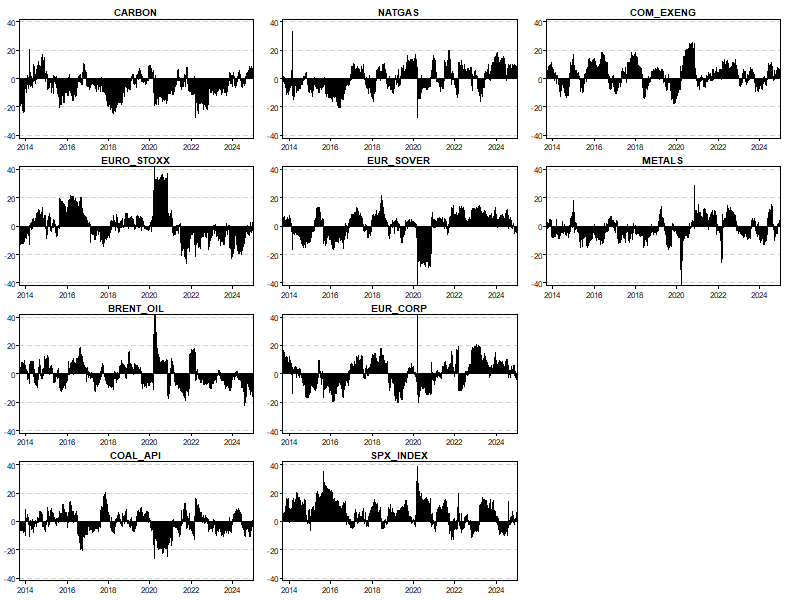
\includegraphics[width = 1.25\linewidth]{8aApdxD-10-180-RetNDC}
      \end{subfigure}
\end{figure}
\begin{figure}[H]
  \ContinuedFloat
  \centering
      \begin{subfigure}[b]{\textwidth}
        \caption{Dynamic volatility net directional connectedness}
        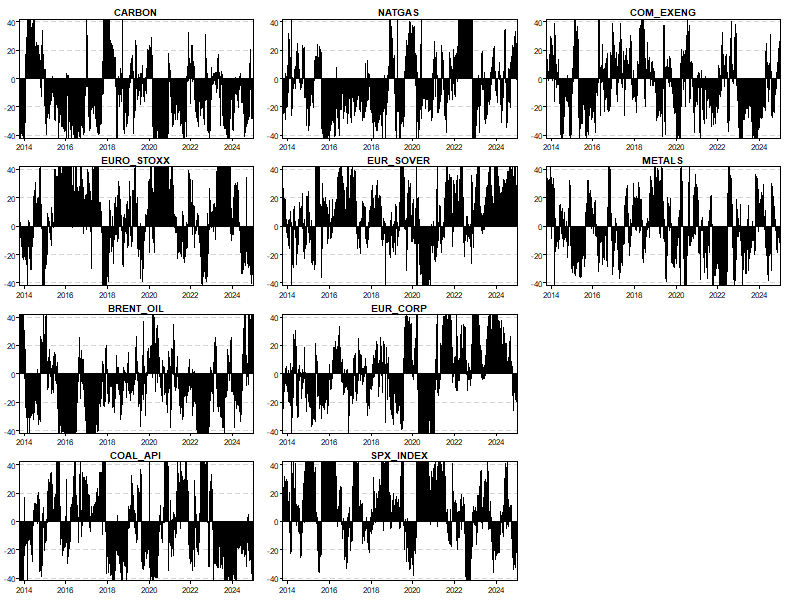
\includegraphics[width = 1.25\linewidth]{8bApdxD-10-180-VolNDC}
      \end{subfigure}
\end{figure}



\subsubsection{Static Return and Volatility Pairwise Directional Connectedness}

\begin{figure}[!ht]
  \caption{Network Representation of Pairwise Connectedness Index (Jan 2013 – Jan 2025)}
  \begin{minipage}{.8\textwidth}
    \subfloat[Static Return PCI network]{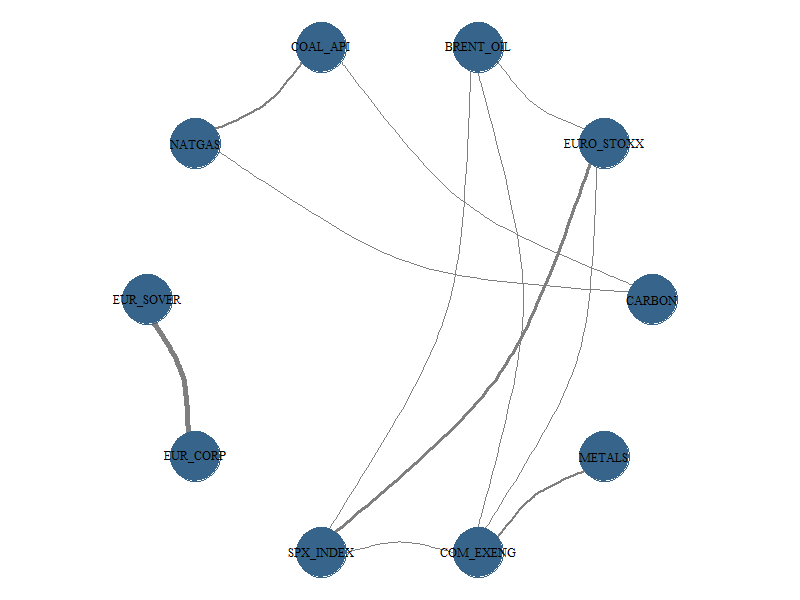
\includegraphics[width = \linewidth]{9aApdxD-10-180-RetNtwrk}}
  \end{minipage}
  \hfill
  \begin{minipage}{.8\textwidth}
    \subfloat[Static Volatility PCI network]{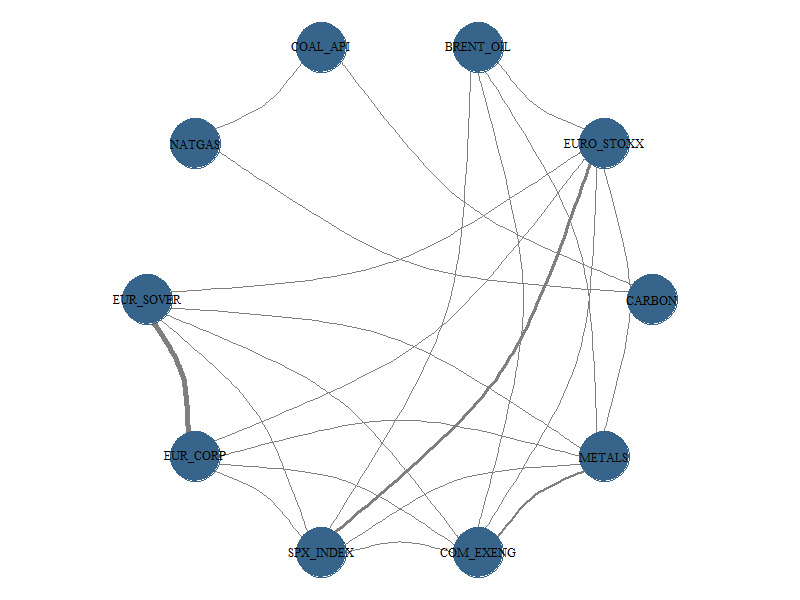
\includegraphics[width = \linewidth]{9bApdxD-10-180-VolNtwrk}}
  \end{minipage}
\end{figure}



\newpage

\subsubsection{Dynamic Return and Volatility Pairwise Directional Connectedness}

\begin{figure}[!ht]
  \caption{Dynamic Return and Volatility Pairwise Connectedness Index (Jan 2013 – Jan 2025)}
  \centering
  \begin{subfigure}[a]{\textwidth}
    \caption{Dynamic return PCI}
    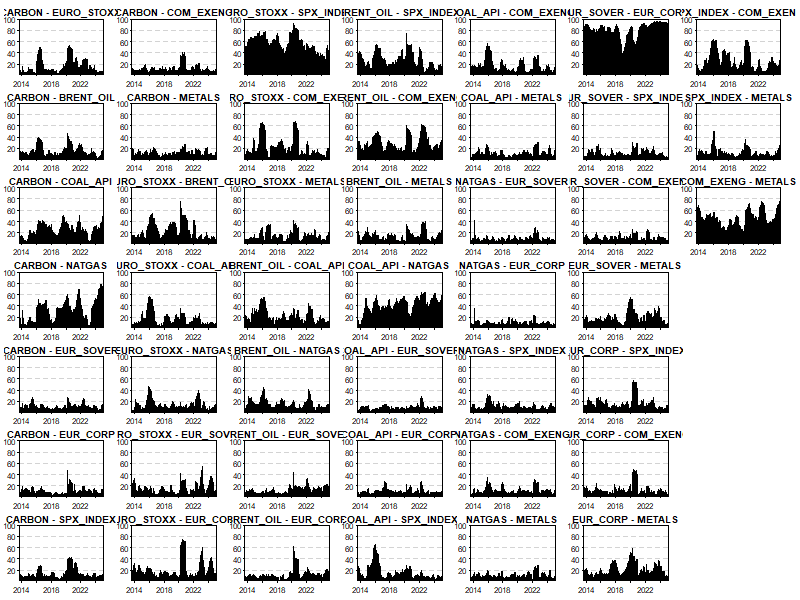
\includegraphics[width = 1.1\linewidth]{10aApdxD-10-180-RetPCI}
  \end{subfigure}
\end{figure}
\begin{figure}[!ht]
  \ContinuedFloat
  \centering
    \begin{subfigure}[b]{\textwidth}\ContinuedFloat
      \caption{Dynamic volatility PCI}
      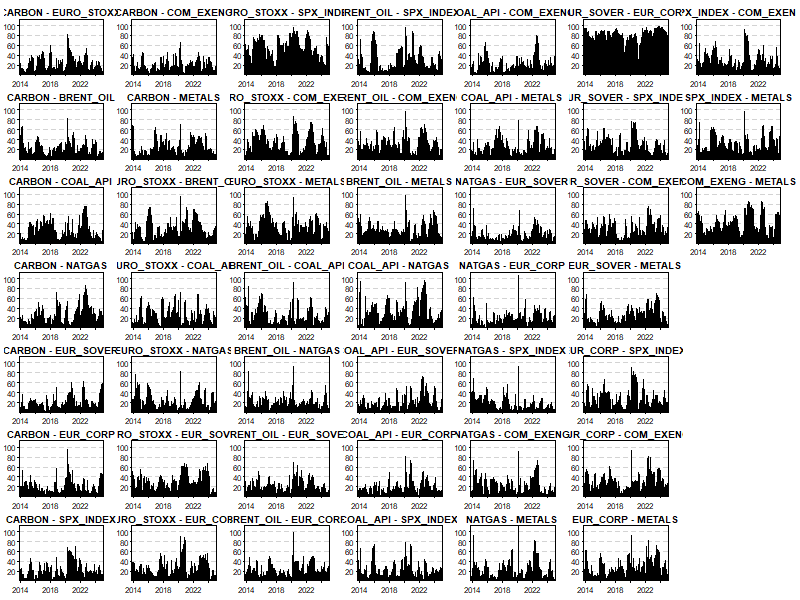
\includegraphics[width = 1.2\linewidth]{10bApdxD-10-180-VolPCI}
    \end{subfigure}
\end{figure}





\subsection{10-period forecast horizon and a rolling window of 220 observations}

\subsubsection{Static Return and Volatility Connectedness Matrix}

  \begin{table}[!ht]
    \caption{Static Return and Volatility Connectedness Matrix (Jan 2013 - Jan 2025)}
      \resizebox{\columnwidth}{!}{
      \begin{tabular}{|l|l|l|l|l|l|l|l|l|l|l|l|}
    \multicolumn{12}{@{}l}{\em(a) Carbon returns connectedness matrix}\\ \hline
        ~ & CARBON & EUROSTOXX & BRENTOIL & COALAPI & NATGAS & EURSOVER & EURCORP & SPXINDEX & COMEXENG & METALS & FROM \\ \hline
        CARBON & 61.35 & 3.93 & 3.67 & 7.77 & 10.07 & 2.29 & 2.12 & 3.28 & 2.6 & 2.91 & 38.65 \\ \hline
        EUROSTOXX & 3.17 & 50.79 & 5.67 & 3.23 & 2.94 & 2.75 & 3.43 & 20.12 & 5.14 & 2.77 & 49.21 \\ \hline
        BRENTOIL & 3.31 & 5.91 & 58.43 & 5.38 & 3.49 & 2.5 & 2.22 & 7.19 & 8.32 & 3.25 & 41.57 \\ \hline
        COALAPI & 6.21 & 3.65 & 5.74 & 57.04 & 13.87 & 1.71 & 1.88 & 3.69 & 3.82 & 2.38 & 42.96 \\ \hline
        NATGAS & 9.8 & 2.86 & 3.74 & 13.76 & 59.97 & 1.62 & 1.6 & 2.23 & 2.37 & 2.05 & 40.03 \\ \hline
        EURSOVER & 1.86 & 2.78 & 2.47 & 1.5 & 1.47 & 49.32 & 32.36 & 2.14 & 1.84 & 4.25 & 50.68 \\ \hline
        EURCORP & 1.83 & 5 & 2.6 & 1.56 & 1.6 & 30.68 & 46.15 & 3.92 & 2.43 & 4.22 & 53.85 \\ \hline
        SPXINDEX & 2.25 & 18.12 & 6.71 & 3.21 & 1.8 & 2.12 & 2.58 & 54.48 & 6.44 & 2.29 & 45.52 \\ \hline
        COMEXENG & 2.32 & 5.03 & 7.42 & 3.34 & 2.17 & 1.96 & 2.21 & 6.63 & 53.93 & 14.98 & 46.07 \\ \hline
        METALS & 2.21 & 2.9 & 2.88 & 2.07 & 2.24 & 4.77 & 5.5 & 2.76 & 16.3 & 58.36 & 41.64 \\ \hline
        DST(TO) & 32.96 & 50.19 & 40.89 & 41.83 & 39.66 & 50.41 & 53.92 & 51.95 & 49.25 & 39.11 & 450.17 \\ \hline
        Inc. Own & 94.31 & 100.98 & 99.31 & 98.87 & 99.63 & 99.74 & 100.08 & 106.43 & 103.18 & 97.48 & cTCI/TCI \\ \hline
        NS (NET) & -5.69 & 0.98 & -0.69 & -1.13 & -0.37 & -0.26 & 0.08 & 6.43 & 3.18 & -2.52 & 50.02/45.02 \\ \hline
    \end{tabular}
    }
    \bigskip
      \resizebox{\columnwidth}{!}{
      \begin{tabular}{|l|l|l|l|l|l|l|l|l|l|l|l|}
    \multicolumn{12}{@{}l}{\em(b) Carbon volatility connectedness matrix}\\ \hline
        ~ & CARBON & EUROSTOXX & BRENTOIL & COALAPI & NATGAS & EURSOVER & EURCORP & SPXINDEX & COMEXENG & METALS & FROM \\ \hline
        CARBON & 57.82 & 4.6 & 3.99 & 7.25 & 6.77 & 3.43 & 3.28 & 4.71 & 3.77 & 4.37 & 42.18 \\ \hline
        EUROSTOXX & 3.26 & 48.44 & 4.96 & 3.2 & 3.12 & 4.95 & 4.06 & 17.08 & 5.26 & 5.68 & 51.56 \\ \hline
        BRENTOIL & 3.71 & 6.49 & 54.56 & 4.78 & 3.39 & 3.48 & 4.09 & 6.32 & 7.29 & 5.9 & 45.44 \\ \hline
        COALAPI & 4.61 & 5.41 & 3.49 & 60.67 & 7.47 & 3.55 & 2.54 & 4.17 & 3 & 5.09 & 39.33 \\ \hline
        NATGAS & 4.33 & 4.33 & 3.04 & 8.15 & 62.01 & 3.2 & 3.63 & 4.47 & 3.24 & 3.6 & 37.99 \\ \hline
        EURSOVER & 1.88 & 6.07 & 3.1 & 2.09 & 1.59 & 46.2 & 25.84 & 5.5 & 3.43 & 4.3 & 53.8 \\ \hline
        EURCORP & 2.48 & 5.69 & 2.46 & 1.93 & 1.95 & 28.91 & 43.34 & 5.93 & 4.14 & 3.17 & 56.66 \\ \hline
        SPXINDEX & 3.03 & 15.53 & 4.64 & 2.83 & 1.51 & 4.32 & 3.72 & 55.36 & 4.18 & 4.88 & 44.64 \\ \hline
        COMEXENG & 2.16 & 7.92 & 4.69 & 3.69 & 3.6 & 4.81 & 4.93 & 6.45 & 51.6 & 10.15 & 48.4 \\ \hline
        METALS & 3.68 & 8.12 & 4.08 & 3.63 & 3.45 & 4.91 & 5.83 & 5.71 & 10.35 & 50.22 & 49.78 \\ \hline
        DST(TO) & 29.15 & 64.17 & 34.46 & 37.57 & 32.84 & 61.55 & 57.91 & 60.35 & 44.66 & 47.14 & 469.8 \\ \hline
        Inc. Own & 86.97 & 112.61 & 89.02 & 98.23 & 94.85 & 107.74 & 101.25 & 115.71 & 96.26 & 97.36 & cTCI/TCI \\ \hline
        NS (NET) & -13.03 & 12.61 & -10.98 & -1.77 & -5.15 & 7.74 & 1.25 & 15.71 & -3.74 & -2.64 & 52.20/46.98 \\ \hline
    \end{tabular}
    }
\end{table}




\subsubsection{Dynamic Return and Volatility Net Directional Connectedness}

\begin{figure}[H]
  \caption{Dynamic Net Directional Connectedness (Jan 2013 – Jan 2025)}
    \centering
      \begin{subfigure}[a]{\textwidth}
        \caption{Dynamic return net directional connectedness}
        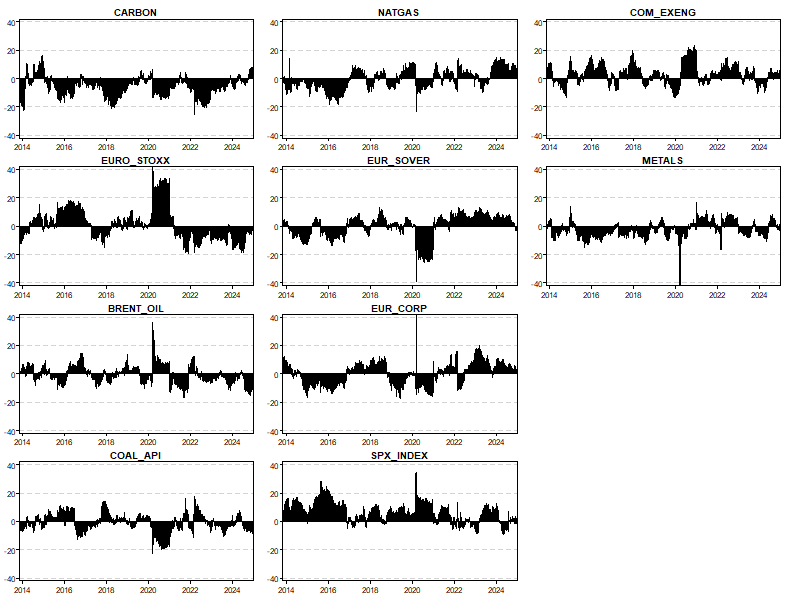
\includegraphics[width = 1.25\linewidth]{11aApdxD-10-220-RetNDC}
      \end{subfigure}
\end{figure}
\begin{figure}[H]
  \ContinuedFloat
  \centering
      \begin{subfigure}[b]{\textwidth}
        \caption{Dynamic volatility net directional connectedness}
        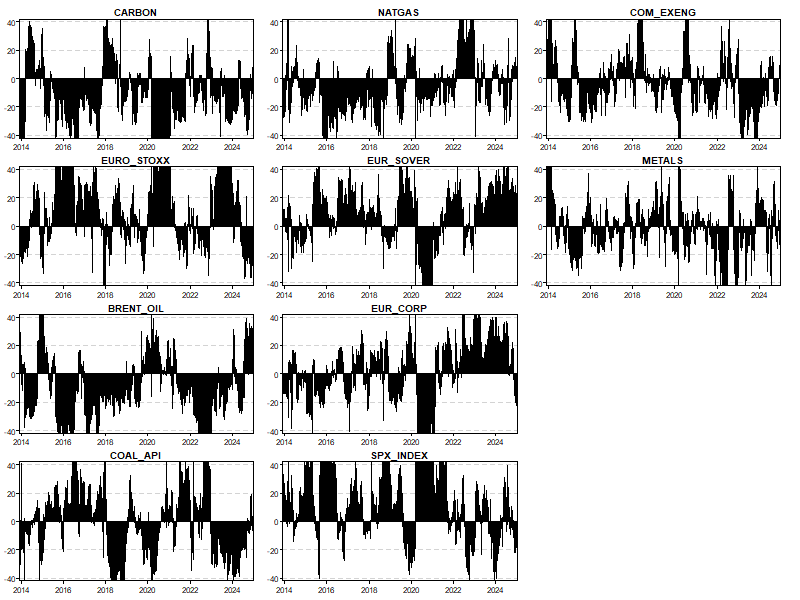
\includegraphics[width = 1.25\linewidth]{11bApdxD-10-220-VolNDC}
      \end{subfigure}
\end{figure}



\subsubsection{Static Return and Volatility Pairwise Directional Connectedness}

\begin{figure}[!ht]
  \caption{Network Representation of Pairwise Connectedness Index (Jan 2013 – Jan 2025)}
  \begin{minipage}{.8\textwidth}
    \subfloat[Static Return PCI network]{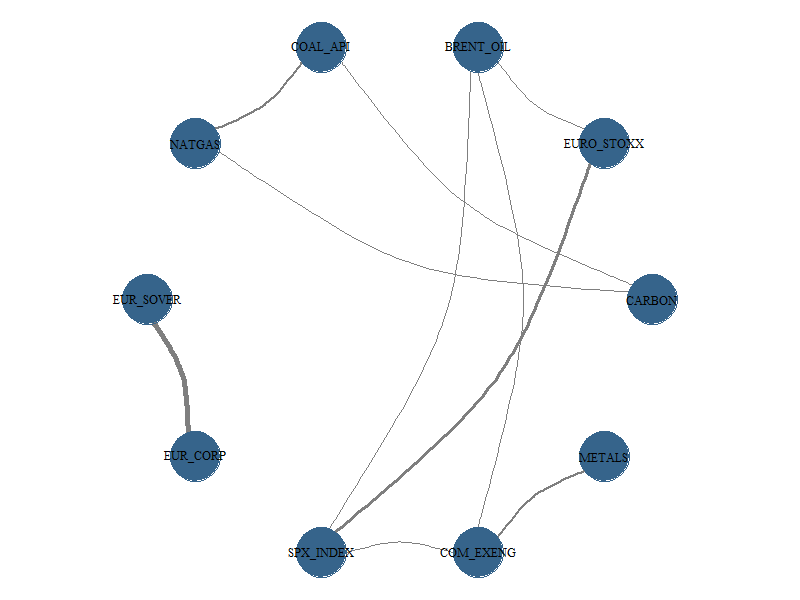
\includegraphics[width = \linewidth]{12aApdxD-10-220-RetNtwrk}}
  \end{minipage}
  \hfill
  \begin{minipage}{.8\textwidth}
    \subfloat[Static Volatility PCI network]{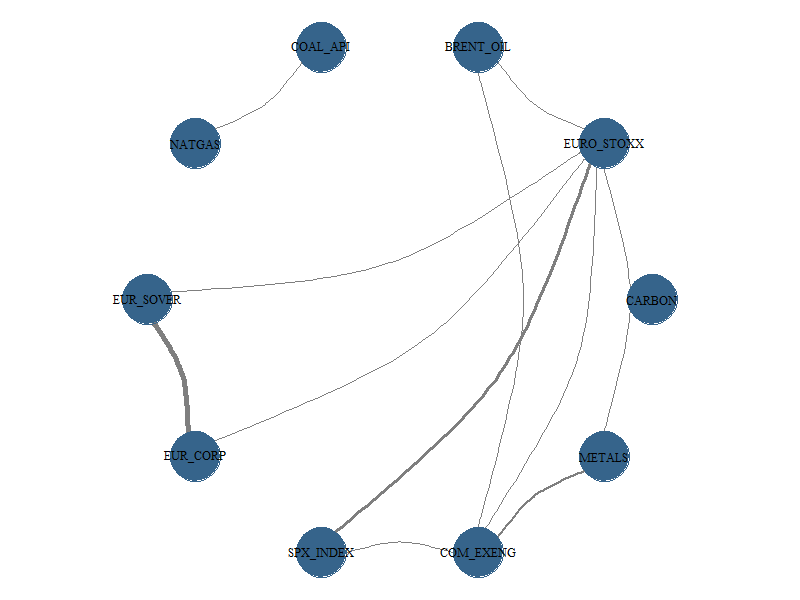
\includegraphics[width = \linewidth]{12bApdxD-10-220-VolNtwrk}}
  \end{minipage}
\end{figure}



\newpage

\subsubsection{Dynamic Return and Volatility Pairwise Directional Connectedness}

\begin{figure}[!ht]
  \caption{Dynamic Return and Volatility Pairwise Connectedness Index (Jan 2013 – Jan 2025)}
  \centering
  \begin{subfigure}[a]{\textwidth}
    \caption{Dynamic return PCI}
    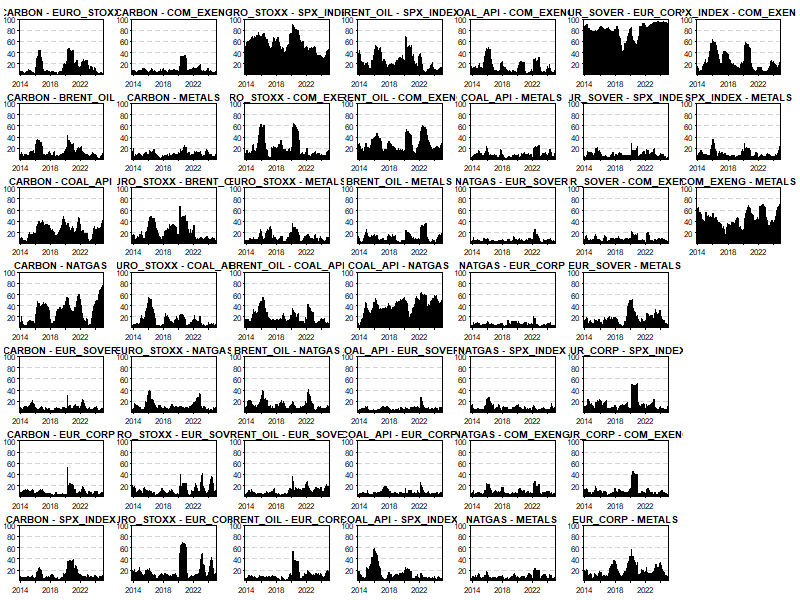
\includegraphics[width = 1.1\linewidth]{13aApdxD-10-220-RetPCI}
  \end{subfigure}
\end{figure}
\begin{figure}[!ht]
  \ContinuedFloat
  \centering
    \begin{subfigure}[b]{\textwidth}\ContinuedFloat
      \caption{Dynamic volatility PCI}
      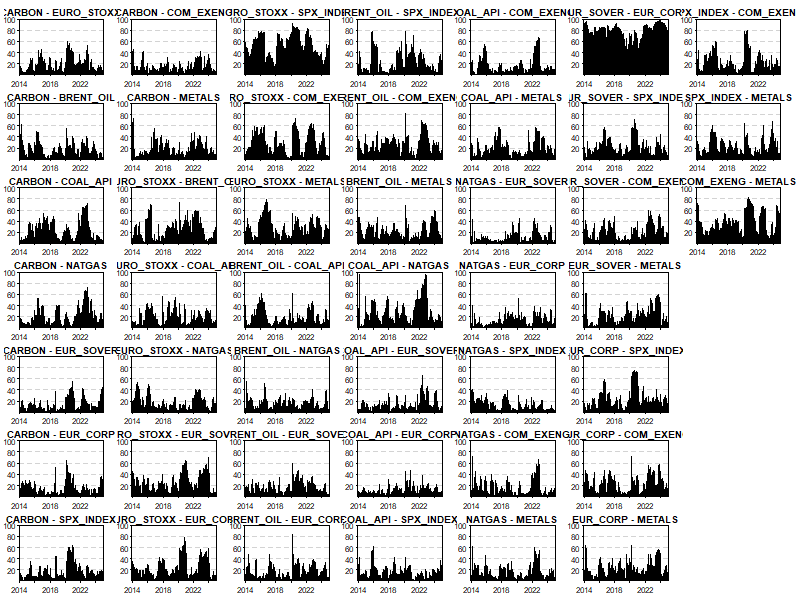
\includegraphics[width = 1.2\linewidth]{13bApdxD-10-220-VolPCI}
    \end{subfigure}
\end{figure}






\subsection{8-period forecast horizon and a rolling window of 180 observations}

\subsubsection{Static Return and Volatility Connectedness Matrix}

  \begin{table}[!ht]
    \caption{Static Return and Volatility Connectedness Matrix (Jan 2013 - Jan 2025)}
      \resizebox{\columnwidth}{!}{   
      \begin{tabular}{|l|l|l|l|l|l|l|l|l|l|l|l|}
      \multicolumn{12}{@{}l}{\em(a) Carbon returns connectedness matrix}\\ \hline
        ~ & CARBON & EUROSTOXX & BRENTOIL & COALAPI & NATGAS & EURSOVER & EURCORP & SPXINDEX & COMEXENG & METALS & FROM \\ \hline
        CARBON & 58.73 & 4.12 & 3.91 & 7.88 & 10.34 & 2.69 & 2.43 & 3.68 & 2.92 & 3.3 & 41.27 \\ \hline
        EUROSTOXX & 3.39 & 48.68 & 5.76 & 3.42 & 3.3 & 3.36 & 3.91 & 19.61 & 5.29 & 3.28 & 51.32 \\ \hline
        BRENTOIL & 3.7 & 6.12 & 56.35 & 5.5 & 3.71 & 2.85 & 2.46 & 7.32 & 8.25 & 3.74 & 43.65 \\ \hline
        COALAPI & 6.46 & 3.9 & 5.87 & 54.95 & 13.64 & 2.04 & 2.22 & 3.99 & 4.08 & 2.87 & 45.05 \\ \hline
        NATGAS & 10.06 & 3.2 & 4.03 & 13.38 & 57.41 & 2.03 & 1.95 & 2.71 & 2.77 & 2.45 & 42.59 \\ \hline
        EURSOVER & 2.21 & 3.22 & 2.9 & 1.85 & 1.87 & 47.39 & 31.45 & 2.41 & 2.25 & 4.43 & 52.61 \\ \hline
        EURCORP & 2.16 & 5.13 & 2.86 & 1.94 & 1.99 & 30.01 & 44.76 & 4.01 & 2.69 & 4.47 & 55.24 \\ \hline
        SPXINDEX & 2.58 & 17.81 & 6.93 & 3.46 & 2.26 & 2.47 & 2.89 & 52.51 & 6.38 & 2.71 & 47.49 \\ \hline
        COMEXENG & 2.66 & 5.13 & 7.45 & 3.6 & 2.65 & 2.37 & 2.51 & 6.56 & 52.2 & 14.86 & 47.8 \\ \hline
        METALS & 2.55 & 3.37 & 3.34 & 2.48 & 2.67 & 4.89 & 5.64 & 3.13 & 15.99 & 55.95 & 44.05 \\ \hline
        DST(TO) & 35.76 & 51.99 & 43.06 & 43.51 & 42.42 & 52.71 & 55.46 & 53.43 & 50.61 & 42.12 & 471.08 \\ \hline
        Inc. Own & 94.5 & 100.68 & 99.41 & 98.45 & 99.83 & 100.1 & 100.22 & 105.94 & 102.81 & 98.07 & cTCI/TCI \\ \hline
        NS (NET) & -5.5 & 0.68 & -0.59 & -1.55 & -0.17 & 0.1 & 0.22 & 5.94 & 2.81 & -1.93 & 52.34/47.11 \\ \hline
    \end{tabular}
    }
    \bigskip
      \resizebox{\columnwidth}{!}{
      \begin{tabular}{|l|l|l|l|l|l|l|l|l|l|l|l|}
    \multicolumn{12}{@{}l}{\em(b) Carbon volatility connectedness matrix}\\ \hline
        ~ & CARBON & EUROSTOXX & BRENTOIL & COALAPI & NATGAS & EURSOVER & EURCORP & SPXINDEX & COMEXENG & METALS & FROM \\ \hline
        CARBON & 57.54 & 4.29 & 4.24 & 6.61 & 7.04 & 3.68 & 3.29 & 4.63 & 3.58 & 5.1 & 42.46 \\ \hline
        EUROSTOXX & 3.64 & 47.92 & 5.2 & 3.73 & 3.31 & 5.24 & 4.1 & 16.18 & 4.86 & 5.81 & 52.08 \\ \hline
        BRENTOIL & 4.54 & 6.27 & 54.13 & 4.66 & 3.32 & 3.65 & 4.43 & 6.37 & 6.68 & 5.96 & 45.87 \\ \hline
        COALAPI & 4.31 & 5.16 & 4.37 & 59.14 & 7.71 & 3.82 & 2.8 & 4.58 & 3.16 & 4.95 & 40.86 \\ \hline
        NATGAS & 4.37 & 4.61 & 3.24 & 7.83 & 61.1 & 3.29 & 3.43 & 4.7 & 3.63 & 3.81 & 38.9 \\ \hline
        EURSOVER & 2.2 & 5.98 & 3.36 & 2.47 & 2.19 & 44.51 & 25.76 & 5.33 & 3.96 & 4.24 & 55.49 \\ \hline
        EURCORP & 2.95 & 5.35 & 2.3 & 2.49 & 2.54 & 28.14 & 42.31 & 5.81 & 4.68 & 3.43 & 57.69 \\ \hline
        SPXINDEX & 3.08 & 15.12 & 5.25 & 2.88 & 1.77 & 4.81 & 4.19 & 53.9 & 4.15 & 4.85 & 46.1 \\ \hline
        COMEXENG & 2.82 & 7.63 & 4.56 & 4.09 & 4.03 & 5.57 & 5.32 & 6.51 & 49.19 & 10.29 & 50.81 \\ \hline
        METALS & 3.96 & 7.74 & 4.37 & 3.92 & 3.82 & 5.1 & 6.4 & 6.17 & 9.52 & 49.01 & 50.99 \\ \hline
        DST(TO) & 31.86 & 62.14 & 36.9 & 38.68 & 35.72 & 63.29 & 59.73 & 60.27 & 44.22 & 48.44 & 481.25 \\ \hline
        Inc. Own & 89.41 & 110.06 & 91.03 & 97.82 & 96.83 & 107.8 & 102.03 & 114.17 & 93.41 & 97.45 & cTCI/TCI \\ \hline
        NS (NET) & -10.59 & 10.06 & -8.97 & -2.18 & -3.17 & 7.8 & 2.03 & 14.17 & -6.59 & -2.55 & 53.47/48.12 \\ \hline
    \end{tabular}
    }
\end{table}




\subsubsection{Dynamic Return and Volatility Net Directional Connectedness}

\begin{figure}[H]
  \caption{Dynamic Net Directional Connectedness (Jan 2013 – Jan 2025)}
    \centering
      \begin{subfigure}[a]{\textwidth}
        \caption{Dynamic return net directional connectedness}
        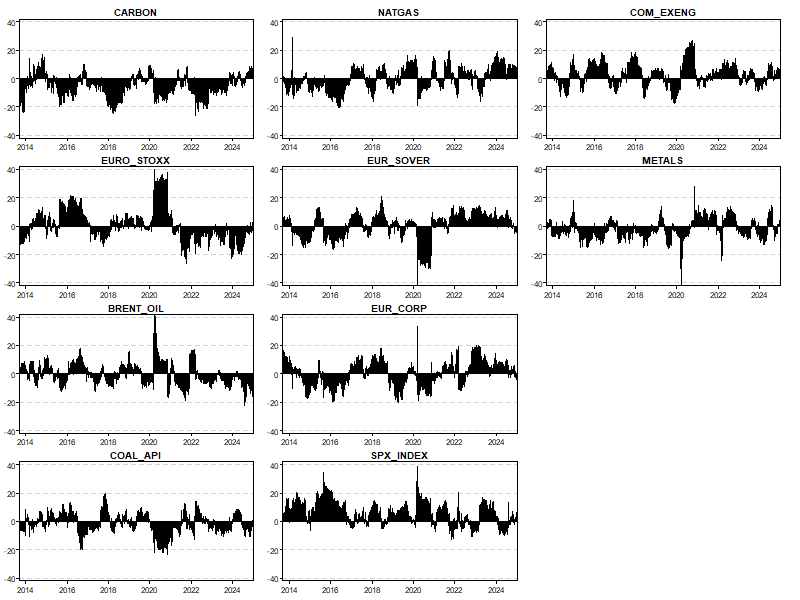
\includegraphics[width = 1.25\linewidth]{14aApdxD-8-180-RetNDC}
      \end{subfigure}
\end{figure}
\begin{figure}[H]
  \ContinuedFloat
  \centering
      \begin{subfigure}[b]{\textwidth}
        \caption{Dynamic volatility net directional connectedness}
        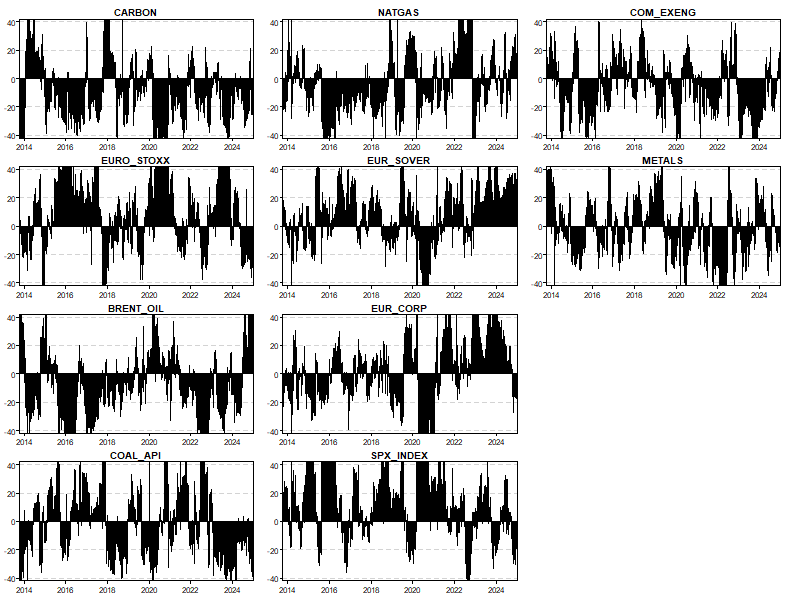
\includegraphics[width = 1.25\linewidth]{14bApdxD-8-180-VolNDC}
      \end{subfigure}
\end{figure}



\subsubsection{Static Return and Volatility Pairwise Directional Connectedness}

\begin{figure}[!ht]
  \caption{Network Representation of Pairwise Connectedness Index (Jan 2013 – Jan 2025)}
  \begin{minipage}{.8\textwidth}
    \subfloat[Static Return PCI network]{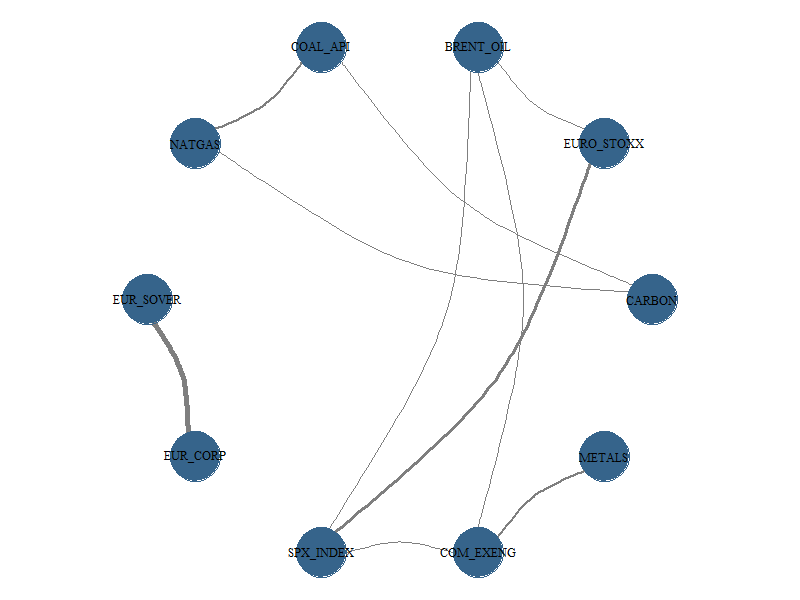
\includegraphics[width = \linewidth]{15aApdxD-8-180-RetNtwrk}}
  \end{minipage}
  \hfill
  \begin{minipage}{.8\textwidth}
    \subfloat[Static Volatility PCI network]{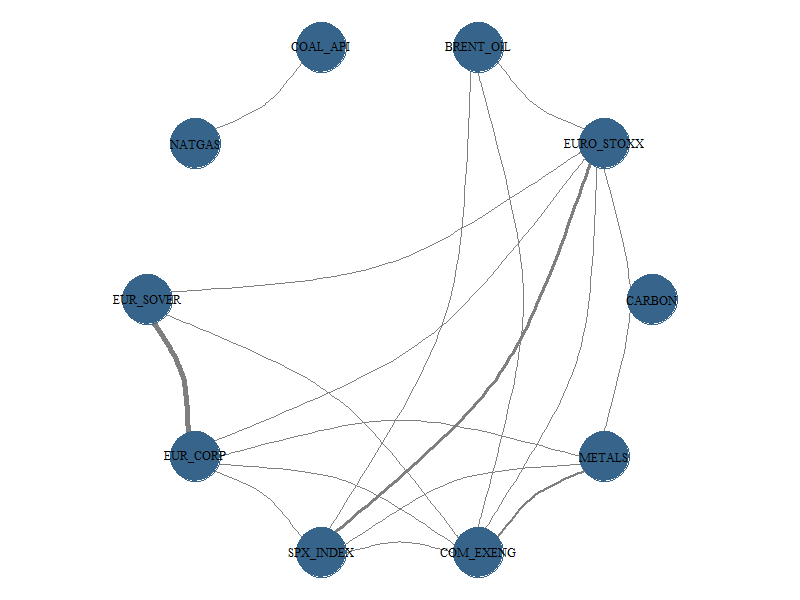
\includegraphics[width = \linewidth]{15bApdxD-8-180-VolNtwrk}}
  \end{minipage}
\end{figure}



\newpage

\subsubsection{Dynamic Return and Volatility Pairwise Directional Connectedness}

\begin{figure}[!ht]
  \caption{Dynamic Return and Volatility Pairwise Connectedness Index (Jan 2013 – Jan 2025)}
  \centering
  \begin{subfigure}[a]{\textwidth}
    \caption{Dynamic return PCI}
    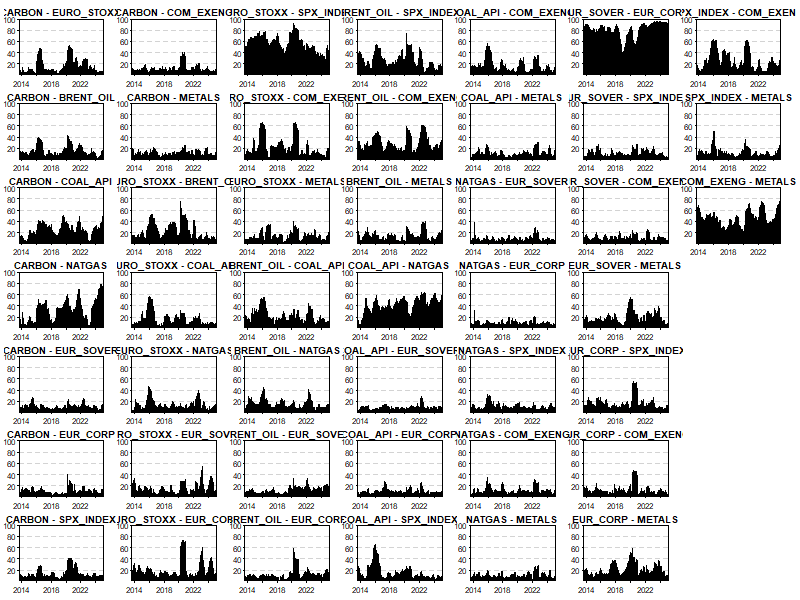
\includegraphics[width = 1.1\linewidth]{16aApdxD-8-180-RetPCI}
  \end{subfigure}
\end{figure}
\begin{figure}[!ht]
  \ContinuedFloat
  \centering
    \begin{subfigure}[b]{\textwidth}\ContinuedFloat
      \caption{Dynamic volatility PCI}
      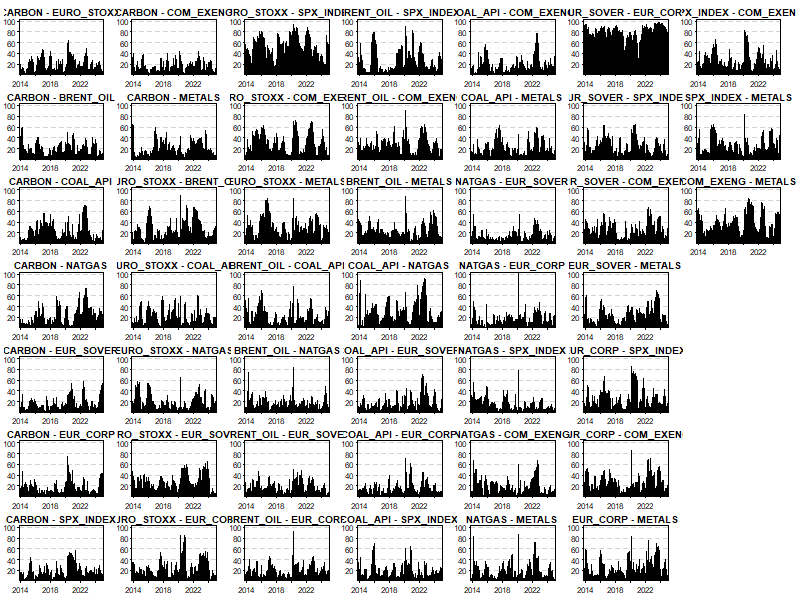
\includegraphics[width = 1.2\linewidth]{16bApdxD-8-180-VolPCI}
    \end{subfigure}
\end{figure}









\subsection{8-period forecast horizon and a rolling window of 200 observations}

\subsubsection{Static Return and Volatility Connectedness Matrix}

  \begin{table}[!ht]
    \caption{Static Return and Volatility Connectedness Matrix (Jan 2013 - Jan 2025)}
      \resizebox{\columnwidth}{!}{
      \begin{tabular}{|l|l|l|l|l|l|l|l|l|l|l|l|}
    \multicolumn{12}{@{}l}{\em(a) Carbon returns connectedness matrix}\\ \hline
        ~ & CARBON & EUROSTOXX & BRENTOIL & COALAPI & NATGAS & EURSOVER & EURCORP & SPXINDEX & COMEXENG & METALS & FROM \\ \hline
        CARBON & 60.33 & 3.99 & 3.77 & 7.83 & 10.23 & 2.42 & 2.21 & 3.44 & 2.72 & 3.05 & 39.67 \\ \hline
        EUROSTOXX & 3.26 & 49.92 & 5.7 & 3.3 & 3.08 & 3.01 & 3.64 & 19.93 & 5.19 & 2.98 & 50.08 \\ \hline
        BRENTOIL & 3.47 & 5.98 & 57.62 & 5.41 & 3.57 & 2.65 & 2.3 & 7.25 & 8.28 & 3.46 & 42.38 \\ \hline
        COALAPI & 6.33 & 3.75 & 5.78 & 56.18 & 13.78 & 1.83 & 2.01 & 3.82 & 3.94 & 2.59 & 43.82 \\ \hline
        NATGAS & 9.94 & 3 & 3.86 & 13.6 & 58.93 & 1.78 & 1.72 & 2.44 & 2.52 & 2.21 & 41.07 \\ \hline
        EURSOVER & 1.99 & 2.97 & 2.64 & 1.64 & 1.63 & 48.54 & 32.01 & 2.25 & 2 & 4.33 & 51.46 \\ \hline
        EURCORP & 1.94 & 5.03 & 2.68 & 1.71 & 1.75 & 30.44 & 45.63 & 3.94 & 2.53 & 4.33 & 54.37 \\ \hline
        SPXINDEX & 2.38 & 17.98 & 6.82 & 3.32 & 2 & 2.25 & 2.7 & 53.68 & 6.39 & 2.47 & 46.32 \\ \hline
        COMEXENG & 2.47 & 5.04 & 7.42 & 3.46 & 2.38 & 2.12 & 2.33 & 6.56 & 53.26 & 14.96 & 46.74 \\ \hline
        METALS & 2.34 & 3.1 & 3.07 & 2.25 & 2.42 & 4.81 & 5.56 & 2.9 & 16.18 & 57.37 & 42.63 \\ \hline
        DST(TO) & 34.12 & 50.84 & 41.75 & 42.53 & 40.82 & 51.31 & 54.49 & 52.53 & 49.76 & 40.39 & 458.54 \\ \hline
        Inc. Own & 94.45 & 100.75 & 99.37 & 98.71 & 99.76 & 99.85 & 100.12 & 106.21 & 103.02 & 97.76 & cTCI/TCI \\ \hline
        NS (NET) & -5.55 & 0.75 & -0.63 & -1.29 & -0.24 & -0.15 & 0.12 & 6.21 & 3.02 & -2.24 & 50.95/45.85 \\ \hline
    \end{tabular}
    }
    \bigskip
      \resizebox{\columnwidth}{!}{
      \begin{tabular}{|l|l|l|l|l|l|l|l|l|l|l|l|}
    \multicolumn{12}{@{}l}{\em(b) Carbon volatility connectedness matrix}\\ \hline
        ~ & CARBON & EUROSTOXX & BRENTOIL & COALAPI & NATGAS & EURSOVER & EURCORP & SPXINDEX & COMEXENG & METALS & FROM \\ \hline
        CARBON & 60.17 & 4.17 & 3.78 & 6.68 & 6.57 & 3.32 & 3.11 & 4.33 & 3.26 & 4.61 & 39.83 \\ \hline
        EUROSTOXX & 3.29 & 49.69 & 5.1 & 3.09 & 2.94 & 4.86 & 3.93 & 16.76 & 4.8 & 5.55 & 50.31 \\ \hline
        BRENTOIL & 4.03 & 6.12 & 56.72 & 4.48 & 3.04 & 3.25 & 4.01 & 6.11 & 6.72 & 5.54 & 43.28 \\ \hline
        COALAPI & 4.14 & 4.95 & 3.92 & 62.24 & 7.35 & 3.39 & 2.39 & 4.07 & 2.83 & 4.7 & 37.76 \\ \hline
        NATGAS & 4.18 & 4.25 & 2.96 & 7.77 & 63.79 & 2.87 & 3.22 & 4.26 & 3.21 & 3.49 & 36.21 \\ \hline
        EURSOVER & 1.94 & 5.82 & 3.08 & 2.1 & 1.74 & 46.3 & 26.28 & 5.1 & 3.44 & 4.21 & 53.7 \\ \hline
        EURCORP & 2.58 & 5.27 & 2.19 & 2.05 & 2.04 & 28.8 & 44.04 & 5.7 & 4.16 & 3.17 & 55.96 \\ \hline
        SPXINDEX & 2.84 & 15.41 & 4.97 & 2.56 & 1.49 & 4.35 & 3.82 & 56.19 & 3.92 & 4.45 & 43.81 \\ \hline
        COMEXENG & 2.32 & 7.68 & 4.52 & 3.73 & 3.57 & 4.87 & 4.97 & 6.12 & 51.84 & 10.37 & 48.16 \\ \hline
        METALS & 3.62 & 7.62 & 4.07 & 3.51 & 3.33 & 4.94 & 5.95 & 5.62 & 9.94 & 51.42 & 48.58 \\ \hline
        DST(TO) & 28.93 & 61.29 & 34.59 & 35.97 & 32.07 & 60.65 & 57.69 & 58.07 & 42.27 & 46.09 & 457.61 \\ \hline
        Inc. Own & 89.1 & 110.98 & 91.3 & 98.21 & 95.85 & 106.95 & 101.73 & 114.26 & 94.11 & 97.51 & cTCI/TCI \\ \hline
        NS (NET) & -10.9 & 10.98 & -8.7 & -1.79 & -4.15 & 6.95 & 1.73 & 14.26 & -5.89 & -2.49 & 50.85/45.76 \\ \hline
    \end{tabular}
    }
\end{table}




\subsubsection{Dynamic Return and Volatility Net Directional Connectedness}

\begin{figure}[H]
  \caption{Dynamic Net Directional Connectedness (Jan 2013 – Jan 2025)}
    \centering
      \begin{subfigure}[a]{\textwidth}
        \caption{Dynamic return net directional connectedness}
        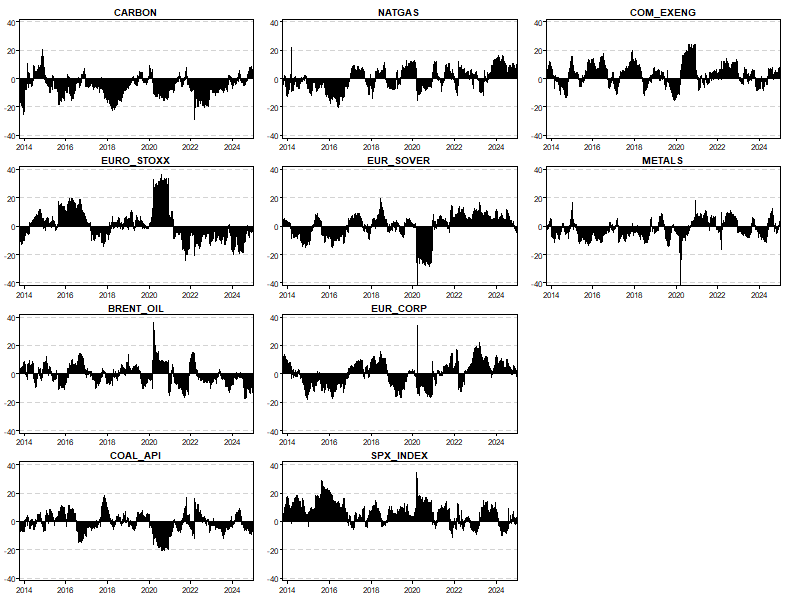
\includegraphics[width = 1.25\linewidth]{17aApdxD-8-200-RetNDC}
      \end{subfigure}
\end{figure}
\begin{figure}[H]
  \ContinuedFloat
  \centering
      \begin{subfigure}[b]{\textwidth}
        \caption{Dynamic volatility net directional connectedness}
        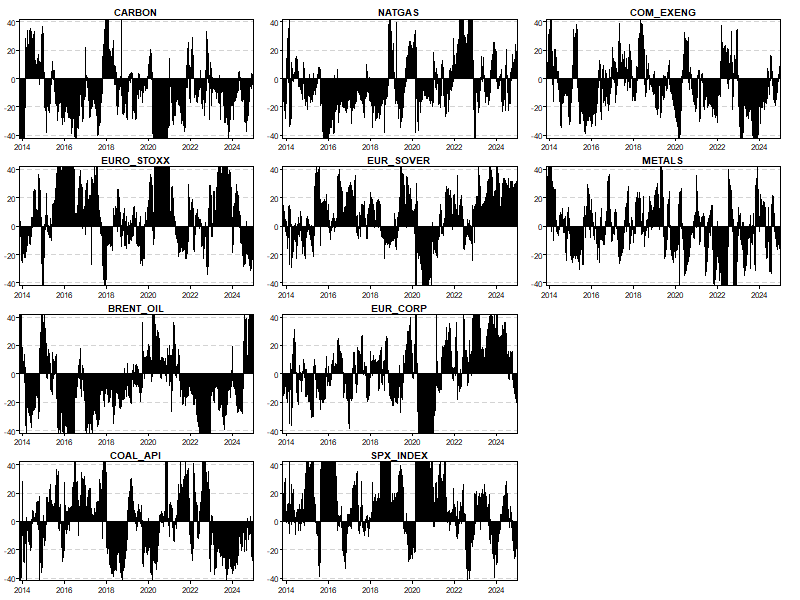
\includegraphics[width = 1.25\linewidth]{17bApdxD-8-200-VolNDC}
      \end{subfigure}
\end{figure}



\subsubsection{Static Return and Volatility Pairwise Directional Connectedness}

\begin{figure}[!ht]
  \caption{Network Representation of Pairwise Connectedness Index (Jan 2013 – Jan 2025)}
  \begin{minipage}{.8\textwidth}
    \subfloat[Static Return PCI network]{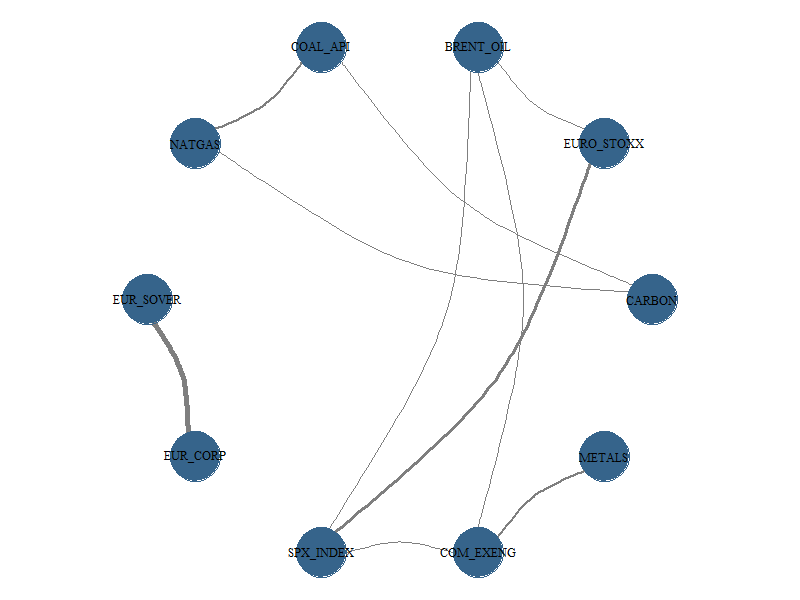
\includegraphics[width = \linewidth]{18aApdxD-8-200-RetNtwrk}}
  \end{minipage}
  \hfill
  \begin{minipage}{.8\textwidth}
    \subfloat[Static Volatility PCI network]{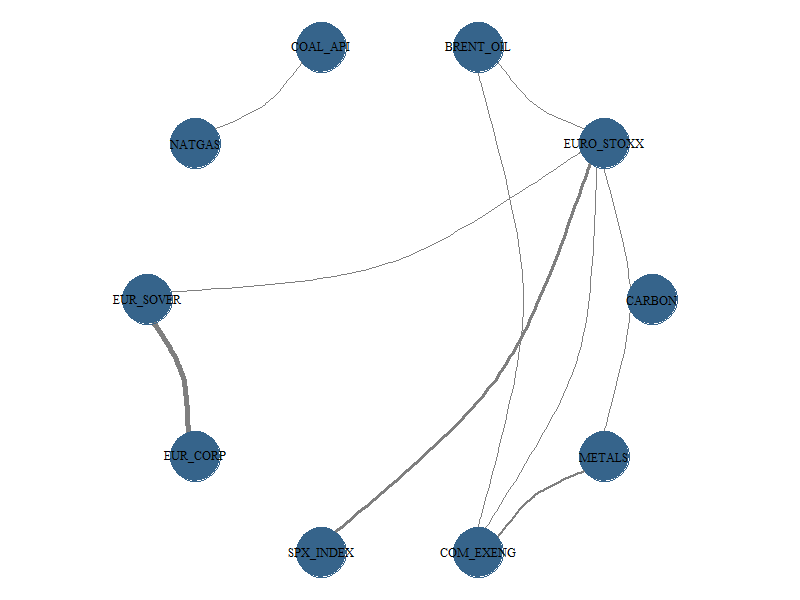
\includegraphics[width = \linewidth]{18bApdxD-8-200-VolNtwrk}}
  \end{minipage}
\end{figure}



\newpage

\subsubsection{Dynamic Return and Volatility Pairwise Directional Connectedness}

\begin{figure}[!ht]
  \caption{Dynamic Return and Volatility Pairwise Connectedness Index (Jan 2013 – Jan 2025)}
  \centering
  \begin{subfigure}[a]{\textwidth}
    \caption{Dynamic return PCI}
    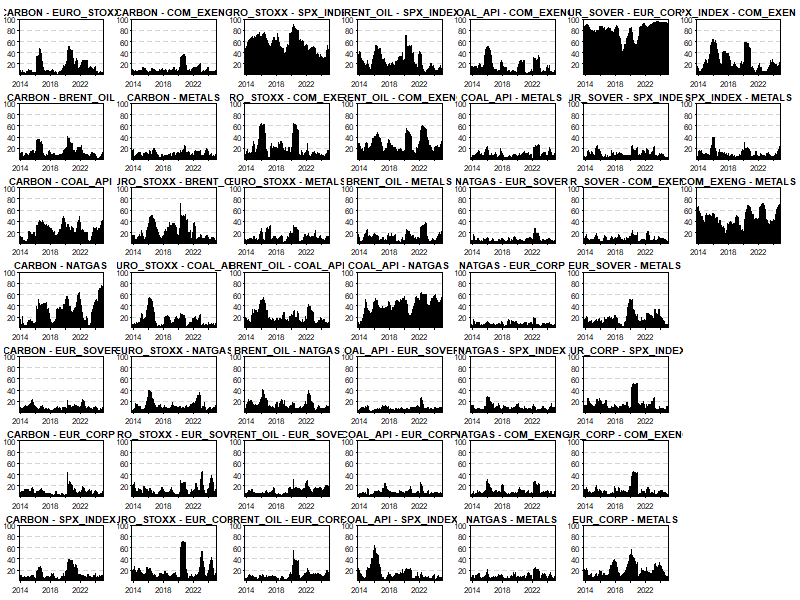
\includegraphics[width = 1.1\linewidth]{19aApdxD-8-200-RetPCI}
  \end{subfigure}
\end{figure}
\begin{figure}[!ht]
  \ContinuedFloat
  \centering
    \begin{subfigure}[b]{\textwidth}\ContinuedFloat
      \caption{Dynamic volatility PCI}
      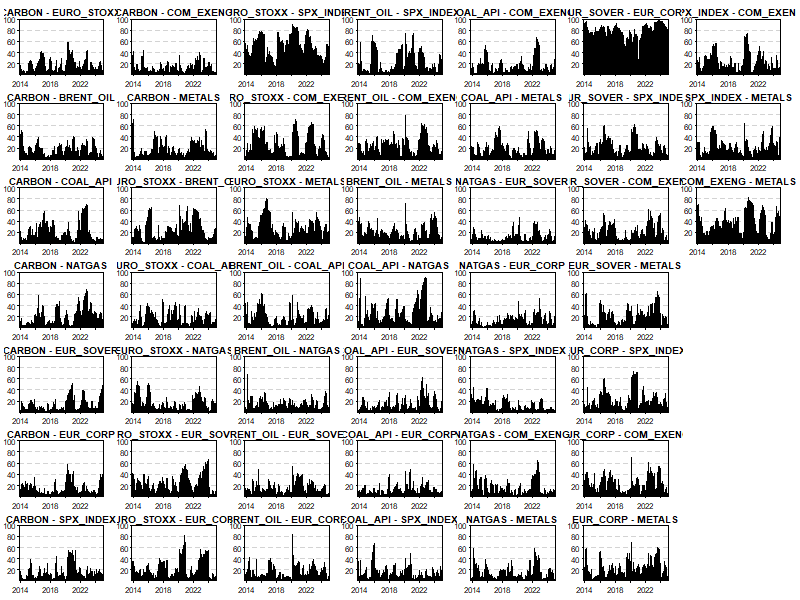
\includegraphics[width = 1.2\linewidth]{19bApdxD-8-200-VolPCI}
    \end{subfigure}
\end{figure}








\subsection{8-period forecast horizon and a rolling window of 220 observations}

\subsubsection{Static Return and Volatility Connectedness Matrix}

  \begin{table}[!ht]
    \caption{Static Return and Volatility Connectedness Matrix (Jan 2013 - Jan 2025)}
      \resizebox{\columnwidth}{!}{
      \begin{tabular}{|l|l|l|l|l|l|l|l|l|l|l|l|}
    \multicolumn{12}{@{}l}{\em(a) Carbon returns connectedness matrix}\\ \hline
        ~ & CARBON & EUROSTOXX & BRENTOIL & COALAPI & NATGAS & EURSOVER & EURCORP & SPXINDEX & COMEXENG & METALS & FROM \\ \hline
        CARBON & 61.59 & 3.93 & 3.64 & 7.76 & 10.08 & 2.24 & 2.07 & 3.26 & 2.57 & 2.86 & 38.41 \\ \hline
        EUROSTOXX & 3.15 & 50.93 & 5.67 & 3.2 & 2.9 & 2.71 & 3.41 & 20.17 & 5.13 & 2.73 & 49.07 \\ \hline
        BRENTOIL & 3.3 & 5.9 & 58.62 & 5.37 & 3.45 & 2.48 & 2.19 & 7.17 & 8.31 & 3.22 & 41.38 \\ \hline
        COALAPI & 6.2 & 3.63 & 5.73 & 57.17 & 13.87 & 1.69 & 1.86 & 3.68 & 3.8 & 2.36 & 42.83 \\ \hline
        NATGAS & 9.8 & 2.83 & 3.73 & 13.77 & 60.14 & 1.6 & 1.57 & 2.19 & 2.34 & 2.03 & 39.86 \\ \hline
        EURSOVER & 1.83 & 2.76 & 2.44 & 1.47 & 1.43 & 49.48 & 32.44 & 2.12 & 1.8 & 4.23 & 50.52 \\ \hline
        EURCORP & 1.81 & 4.98 & 2.57 & 1.53 & 1.55 & 30.74 & 46.27 & 3.9 & 2.43 & 4.21 & 53.73 \\ \hline
        SPXINDEX & 2.22 & 18.15 & 6.71 & 3.18 & 1.78 & 2.07 & 2.56 & 54.62 & 6.44 & 2.26 & 45.38 \\ \hline
        COMEXENG & 2.31 & 4.99 & 7.41 & 3.32 & 2.15 & 1.93 & 2.17 & 6.6 & 54.09 & 15.02 & 45.91 \\ \hline
        METALS & 2.19 & 2.85 & 2.84 & 2.05 & 2.2 & 4.76 & 5.48 & 2.69 & 16.34 & 58.6 & 41.4 \\ \hline
        DST(TO) & 32.81 & 50.03 & 40.74 & 41.65 & 39.42 & 50.23 & 53.75 & 51.77 & 49.15 & 38.94 & 448.48 \\ \hline
        Inc. Own & 94.4 & 100.96 & 99.36 & 98.83 & 99.56 & 99.71 & 100.02 & 106.39 & 103.24 & 97.54 & cTCI/TCI \\ \hline
        NS (NET) & -5.6 & 0.96 & -0.64 & -1.17 & -0.44 & -0.29 & 0.02 & 6.39 & 3.24 & -2.46 & 49.83/44.85 \\ \hline
    \end{tabular}
    }
    \bigskip
      \resizebox{\columnwidth}{!}{
      \begin{tabular}{|l|l|l|l|l|l|l|l|l|l|l|l|}
    \multicolumn{12}{@{}l}{\em(b) Carbon volatility connectedness matrix}\\ \hline
        ~ & CARBON & EUROSTOXX & BRENTOIL & COALAPI & NATGAS & EURSOVER & EURCORP & SPXINDEX & COMEXENG & METALS & FROM \\ \hline
        CARBON & 62.2 & 4.14 & 3.49 & 6.68 & 6.23 & 3.06 & 2.83 & 4.04 & 3.14 & 4.2 & 37.8 \\ \hline
        EUROSTOXX & 2.95 & 50.86 & 4.93 & 2.73 & 2.66 & 4.69 & 3.87 & 17.15 & 4.84 & 5.33 & 49.14 \\ \hline
        BRENTOIL & 3.56 & 6.04 & 58.65 & 4.31 & 2.84 & 2.92 & 3.59 & 5.91 & 6.93 & 5.24 & 41.35 \\ \hline
        COALAPI & 4.12 & 4.62 & 3.28 & 64.8 & 7 & 3.13 & 2.22 & 3.66 & 2.66 & 4.52 & 35.2 \\ \hline
        NATGAS & 4.07 & 3.96 & 2.61 & 7.59 & 66.13 & 2.57 & 3.05 & 3.93 & 2.92 & 3.16 & 33.87 \\ \hline
        EURSOVER & 1.71 & 5.66 & 2.88 & 1.82 & 1.5 & 47.64 & 26.63 & 4.99 & 3.08 & 4.09 & 52.36 \\ \hline
        EURCORP & 2.3 & 5.25 & 2.14 & 1.71 & 1.66 & 29.27 & 45.3 & 5.68 & 3.66 & 3.02 & 54.7 \\ \hline
        SPXINDEX & 2.61 & 15.47 & 4.61 & 2.36 & 1.32 & 4.01 & 3.62 & 58.11 & 3.72 & 4.17 & 41.89 \\ \hline
        COMEXENG & 1.91 & 7.65 & 4.54 & 3.52 & 3.19 & 4.42 & 4.56 & 5.92 & 53.86 & 10.43 & 46.14 \\ \hline
        METALS & 3.41 & 7.37 & 3.76 & 3.24 & 2.95 & 4.79 & 5.5 & 5.17 & 10.24 & 53.57 & 46.43 \\ \hline
        DST(TO) & 26.64 & 60.17 & 32.23 & 33.96 & 29.35 & 58.88 & 55.87 & 56.45 & 41.18 & 44.17 & 438.89 \\ \hline
        Inc. Own & 88.84 & 111.02 & 90.88 & 98.75 & 95.49 & 106.52 & 101.17 & 114.56 & 95.04 & 97.73 & cTCI/TCI \\ \hline
        NS (NET) & -11.16 & 11.02 & -9.12 & -1.25 & -4.51 & 6.52 & 1.17 & 14.56 & -4.96 & -2.27 & 48.77/43.89 \\ \hline
    \end{tabular}
    }
\end{table}




\subsubsection{Dynamic Return and Volatility Net Directional Connectedness}

\begin{figure}[H]
  \caption{Dynamic Net Directional Connectedness (Jan 2013 – Jan 2025)}
    \centering
      \begin{subfigure}[a]{\textwidth}
        \caption{Dynamic return net directional connectedness}
        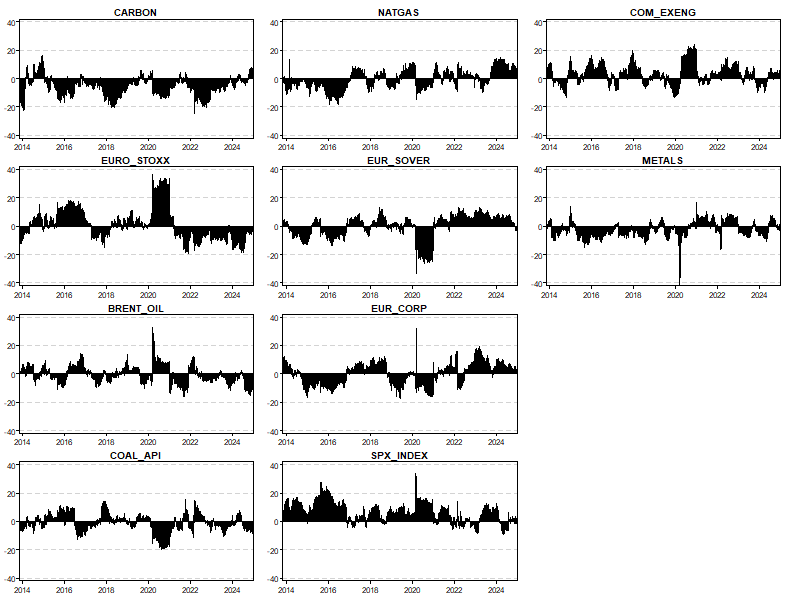
\includegraphics[width = 1.25\linewidth]{20aApdxD-8-220-RetNDC}
      \end{subfigure}
\end{figure}
\begin{figure}[H]
  \ContinuedFloat
  \centering
      \begin{subfigure}[b]{\textwidth}
        \caption{Dynamic volatility net directional connectedness}
        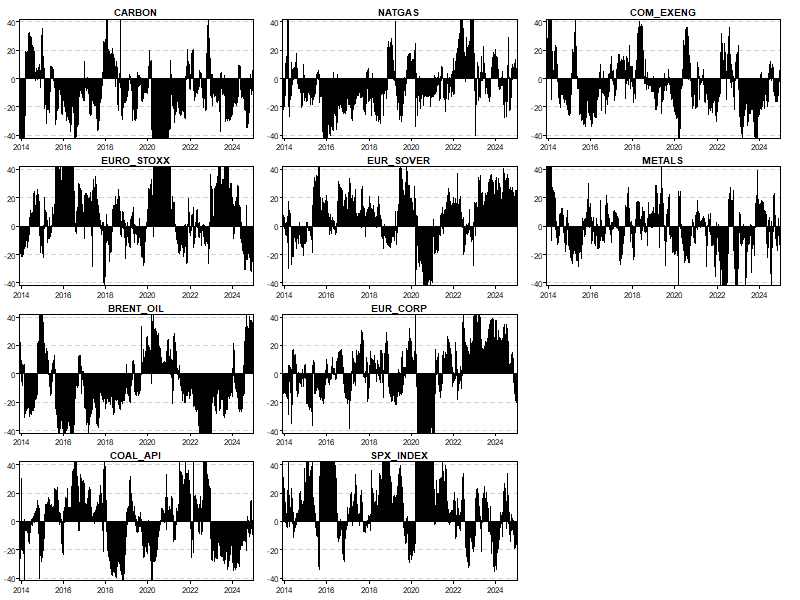
\includegraphics[width = 1.25\linewidth]{20bApdxD-8-220-VolNDC}
      \end{subfigure}
\end{figure}



\subsubsection{Static Return and Volatility Pairwise Directional Connectedness}

\begin{figure}[!ht]
  \caption{Network Representation of Pairwise Connectedness Index (Jan 2013 – Jan 2025)}
  \begin{minipage}{.8\textwidth}
    \subfloat[Static Return PCI network]{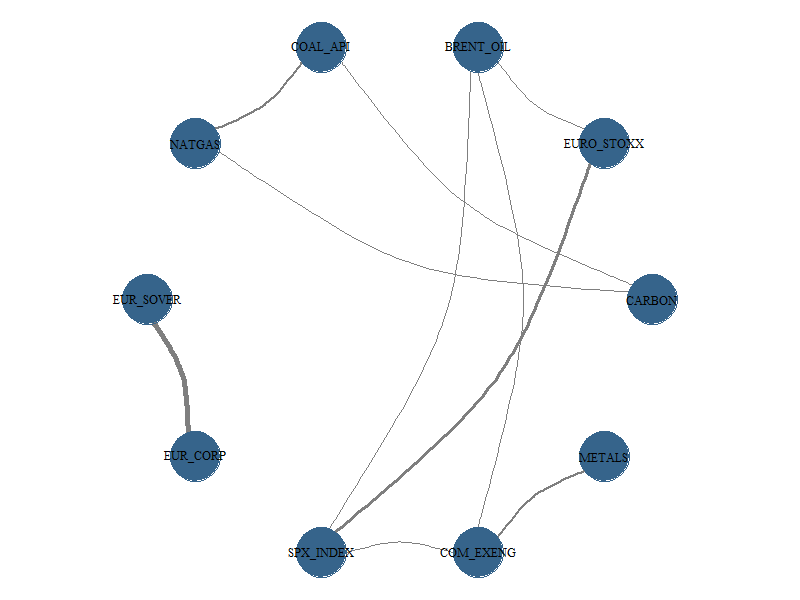
\includegraphics[width = \linewidth]{21aApdxD-8-220-RetNtwrk}}
  \end{minipage}
  \hfill
  \begin{minipage}{.8\textwidth}
    \subfloat[Static Volatility PCI network]{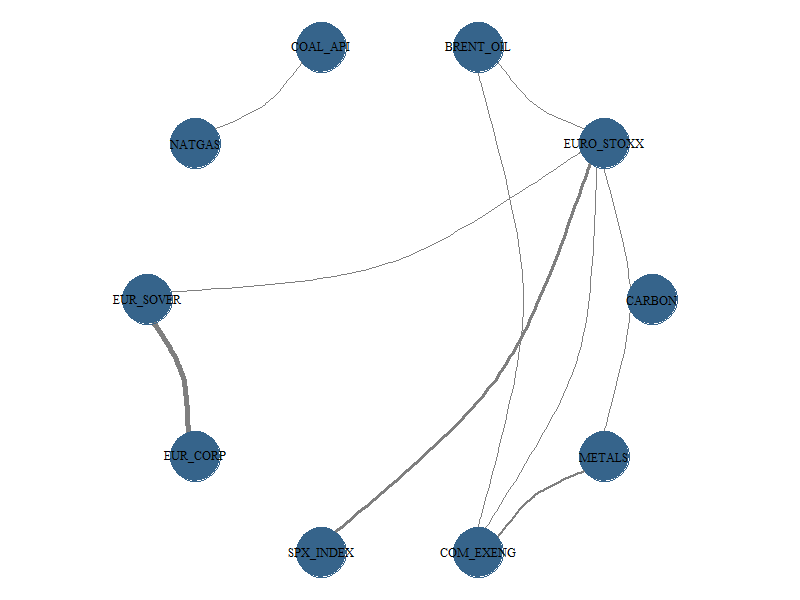
\includegraphics[width = \linewidth]{21bApdxD-8-220-VolNtwrk}}
  \end{minipage}
\end{figure}



\newpage

\subsubsection{Dynamic Return and Volatility Pairwise Directional Connectedness}

\begin{figure}[!ht]
  \caption{Dynamic Return and Volatility Pairwise Connectedness Index (Jan 2013 – Jan 2025)}
  \centering
  \begin{subfigure}[a]{\textwidth}
    \caption{Dynamic return PCI}
    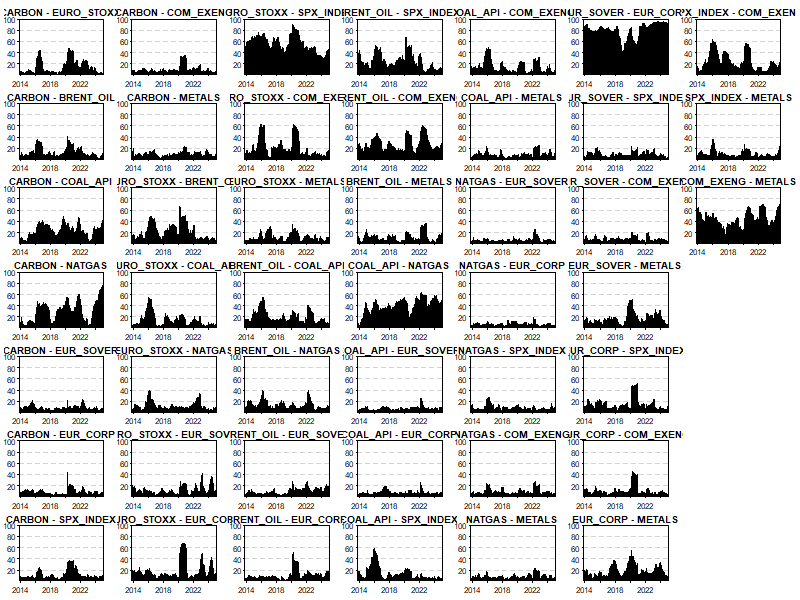
\includegraphics[width = 1.1\linewidth]{22aApdxD-8-220-RetPCI}
  \end{subfigure}
\end{figure}
\begin{figure}[!ht]
  \ContinuedFloat
  \centering
    \begin{subfigure}[b]{\textwidth}\ContinuedFloat
      \caption{Dynamic volatility PCI}
      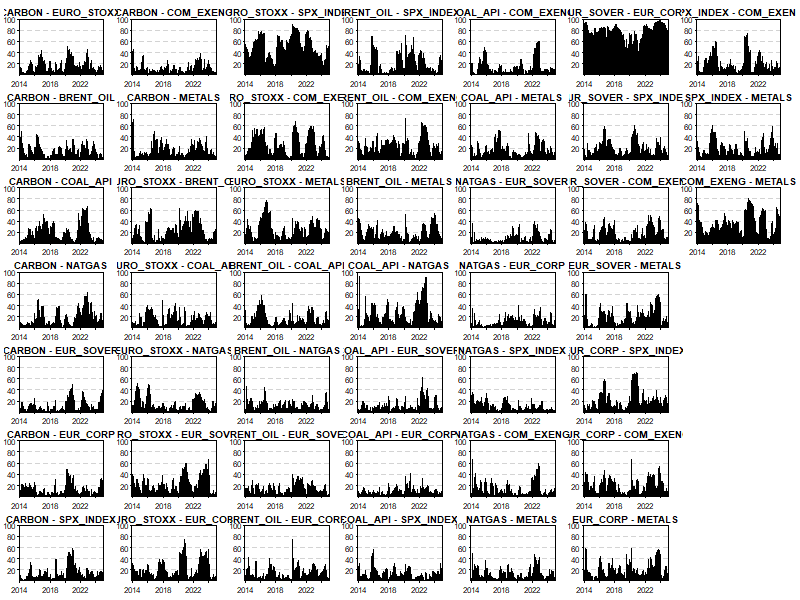
\includegraphics[width = 1.2\linewidth]{22bApdxD-8-220-VolPCI}
    \end{subfigure}
\end{figure}










\subsection{12-period forecast horizon and a rolling window of 180 observations}

\subsubsection{Static Return and Volatility Connectedness Matrix}

  \begin{table}[!ht]
    \caption{Static Return and Volatility Connectedness Matrix (Jan 2013 - Jan 2025)}
      \resizebox{\columnwidth}{!}{
      \begin{tabular}{|l|l|l|l|l|l|l|l|l|l|l|l|}
    \multicolumn{12}{@{}l}{\em(a) Carbon returns connectedness matrix}\\ \hline
        ~ & CARBON & EUROSTOXX & BRENTOIL & COALAPI & NATGAS & EURSOVER & EURCORP & SPXINDEX & COMEXENG & METALS & FROM \\ \hline
        CARBON & 58.33 & 4.13 & 3.97 & 7.9 & 10.32 & 2.77 & 2.5 & 3.72 & 2.98 & 3.39 & 41.67 \\ \hline
        EUROSTOXX & 3.43 & 48.44 & 5.78 & 3.45 & 3.36 & 3.41 & 3.95 & 19.53 & 5.31 & 3.33 & 51.56 \\ \hline
        BRENTOIL & 3.74 & 6.15 & 55.99 & 5.54 & 3.77 & 2.9 & 2.52 & 7.35 & 8.26 & 3.79 & 44.01 \\ \hline
        COALAPI & 6.48 & 3.93 & 5.89 & 54.66 & 13.62 & 2.09 & 2.26 & 4.03 & 4.12 & 2.93 & 45.34 \\ \hline
        NATGAS & 10.05 & 3.25 & 4.07 & 13.36 & 57.07 & 2.08 & 2.01 & 2.78 & 2.84 & 2.5 & 42.93 \\ \hline
        EURSOVER & 2.27 & 3.27 & 2.96 & 1.9 & 1.95 & 47.08 & 31.3 & 2.47 & 2.32 & 4.48 & 52.92 \\ \hline
        EURCORP & 2.19 & 5.15 & 2.91 & 1.99 & 2.07 & 29.9 & 44.54 & 4.04 & 2.71 & 4.5 & 55.46 \\ \hline
        SPXINDEX & 2.63 & 17.76 & 6.94 & 3.51 & 2.3 & 2.54 & 2.93 & 52.24 & 6.4 & 2.76 & 47.76 \\ \hline
        COMEXENG & 2.69 & 5.18 & 7.48 & 3.64 & 2.69 & 2.43 & 2.57 & 6.6 & 51.91 & 14.81 & 48.09 \\ \hline
        METALS & 2.58 & 3.45 & 3.41 & 2.53 & 2.74 & 4.92 & 5.68 & 3.22 & 15.92 & 55.54 & 44.46 \\ \hline
        DST(TO) & 36.06 & 52.28 & 43.39 & 43.82 & 42.82 & 53.03 & 55.73 & 53.74 & 50.85 & 42.49 & 474.2 \\ \hline
        Inc. Own & 94.39 & 100.72 & 99.38 & 98.47 & 99.89 & 100.11 & 100.27 & 105.98 & 102.76 & 98.03 & cTCI/TCI \\ \hline
        NS (NET) & -5.61 & 0.72 & -0.62 & -1.53 & -0.11 & 0.11 & 0.27 & 5.98 & 2.76 & -1.97 & 52.69/47.42 \\ \hline
    \end{tabular}
    }
    \bigskip
      \resizebox{\columnwidth}{!}{
    \begin{tabular}{|l|l|l|l|l|l|l|l|l|l|l|l|}
    \multicolumn{12}{@{}l}{\em(b) Carbon volatility connectedness matrix}\\ \hline
        ~ & CARBON & EUROSTOXX & BRENTOIL & COALAPI & NATGAS & EURSOVER & EURCORP & SPXINDEX & COMEXENG & METALS & FROM \\ \hline
        CARBON & 49.07 & 5.05 & 5.04 & 7.53 & 8.1 & 4.71 & 4.25 & 6.24 & 4.55 & 5.47 & 50.93 \\ \hline
        EUROSTOXX & 4.34 & 42.48 & 5.5 & 4.66 & 4.47 & 5.91 & 4.68 & 15.49 & 5.76 & 6.72 & 57.52 \\ \hline
        BRENTOIL & 4.91 & 7.05 & 46.16 & 5.52 & 4.3 & 4.89 & 5.5 & 7.04 & 7.5 & 7.13 & 53.84 \\ \hline
        COALAPI & 5.42 & 6.83 & 4.96 & 50.79 & 8.67 & 4.61 & 3.48 & 5.51 & 3.82 & 5.91 & 49.21 \\ \hline
        NATGAS & 5.12 & 5.38 & 4.23 & 8.78 & 52.69 & 4.47 & 4.44 & 5.78 & 4.38 & 4.72 & 47.31 \\ \hline
        EURSOVER & 2.74 & 6.84 & 3.83 & 3.16 & 2.59 & 41.18 & 23.89 & 6.2 & 4.83 & 4.75 & 58.82 \\ \hline
        EURCORP & 3.51 & 6.06 & 2.89 & 3.07 & 3.37 & 26.97 & 38.08 & 6.43 & 5.71 & 3.9 & 61.92 \\ \hline
        SPXINDEX & 4 & 14.79 & 5.55 & 3.89 & 2.41 & 5.65 & 4.67 & 47.45 & 5.22 & 6.37 & 52.55 \\ \hline
        COMEXENG & 3.54 & 8.03 & 4.9 & 4.53 & 4.92 & 6.48 & 6.13 & 7.47 & 44.23 & 9.77 & 55.77 \\ \hline
        METALS & 4.45 & 8.84 & 5.11 & 4.64 & 4.75 & 5.52 & 7.13 & 7.41 & 9.82 & 42.32 & 57.68 \\ \hline
        DST(TO) & 38.03 & 68.87 & 42.02 & 45.78 & 43.58 & 69.22 & 64.17 & 67.57 & 51.57 & 54.74 & 545.55 \\ \hline
        Inc. Own & 87.1 & 111.35 & 88.18 & 96.57 & 96.27 & 110.4 & 102.26 & 115.01 & 95.8 & 97.06 & cTCI/TCI \\ \hline
        NS (NET) & -12.9 & 11.35 & -11.82 & -3.43 & -3.73 & 10.4 & 2.26 & 15.01 & -4.2 & -2.94 & 60.62/54.55 \\ \hline
    \end{tabular}
    }
\end{table}




\subsubsection{Dynamic Return and Volatility Net Directional Connectedness}

\begin{figure}[H]
  \caption{Dynamic Net Directional Connectedness (Jan 2013 – Jan 2025)}
    \centering
      \begin{subfigure}[a]{\textwidth}
        \caption{Dynamic return net directional connectedness}
        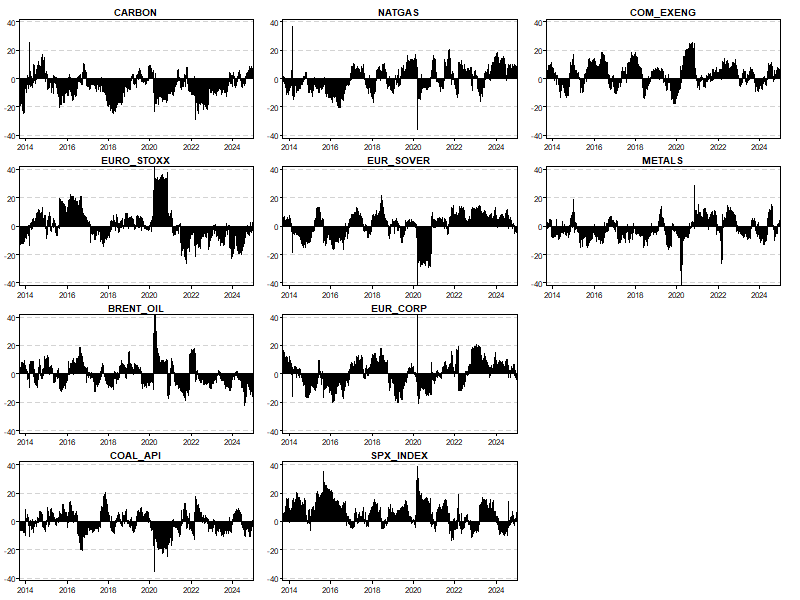
\includegraphics[width = 1.25\linewidth]{23aApdxD-12-180-RetNDC}
      \end{subfigure}
\end{figure}
\begin{figure}[H]
  \ContinuedFloat
  \centering
      \begin{subfigure}[b]{\textwidth}
        \caption{Dynamic volatility net directional connectedness}
        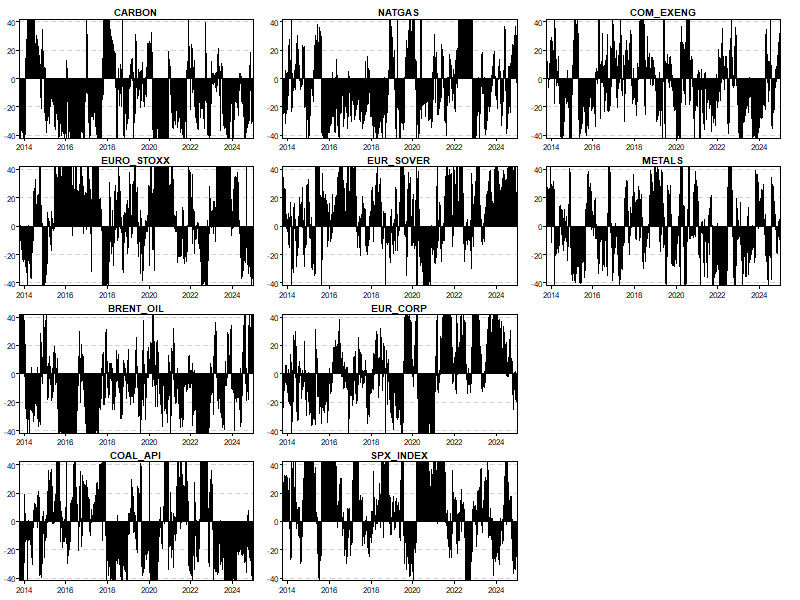
\includegraphics[width = 1.25\linewidth]{23bApdxD-12-180-VolNDC}
      \end{subfigure}
\end{figure}



\subsubsection{Static Return and Volatility Pairwise Directional Connectedness}

\begin{figure}[!ht]
  \caption{Network Representation of Pairwise Connectedness Index (Jan 2013 – Jan 2025)}
  \begin{minipage}{.8\textwidth}
    \subfloat[Static Return PCI network]{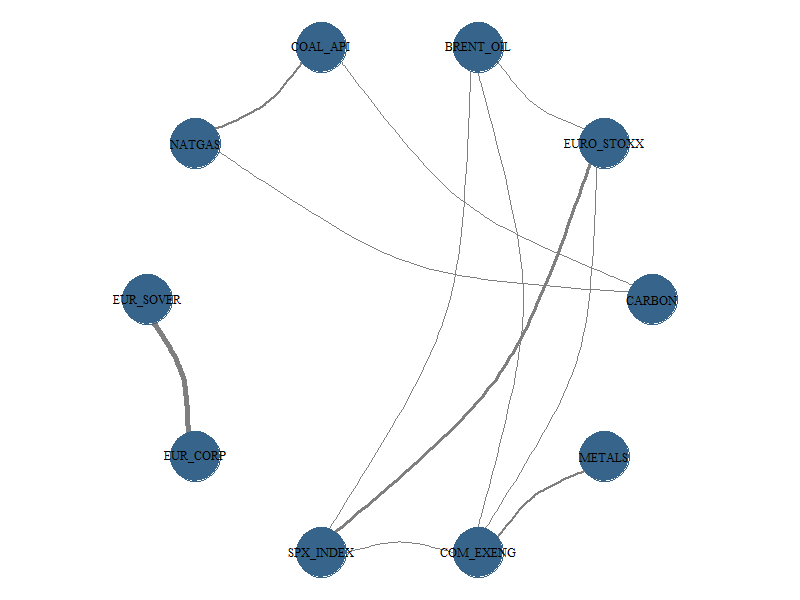
\includegraphics[width = \linewidth]{24aApdxD-12-180-RetNtwrk}}
  \end{minipage}
  \hfill
  \begin{minipage}{.8\textwidth}
    \subfloat[Static Volatility PCI network]{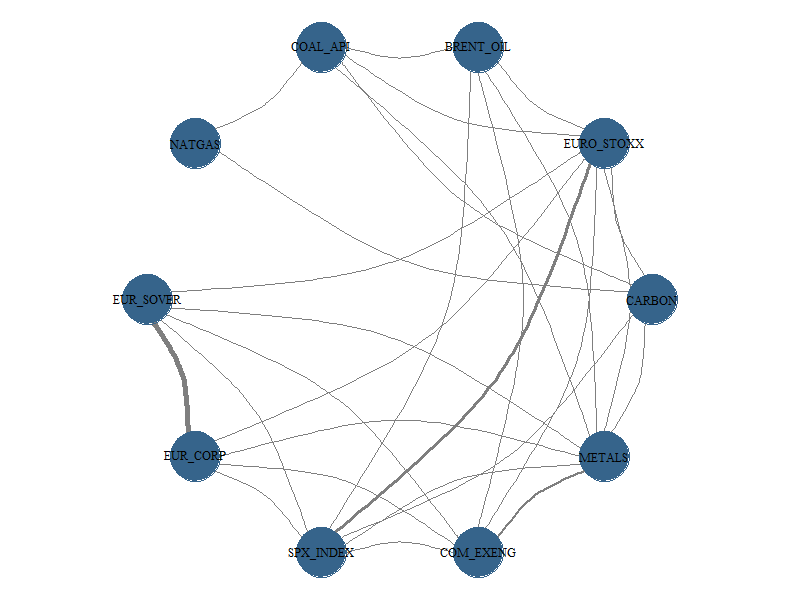
\includegraphics[width = \linewidth]{24bApdxD-12-180-VolNtwrk}}
  \end{minipage}
\end{figure}



\newpage

\subsubsection{Dynamic Return and Volatility Pairwise Directional Connectedness}

\begin{figure}[!ht]
  \caption{Dynamic Return and Volatility Pairwise Connectedness Index (Jan 2013 – Jan 2025)}
  \centering
  \begin{subfigure}[a]{\textwidth}
    \caption{Dynamic return PCI}
    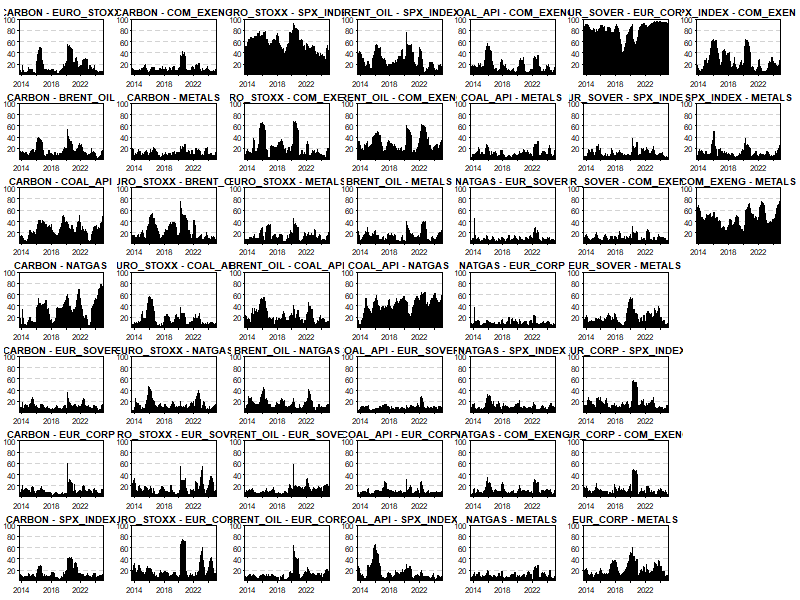
\includegraphics[width = 1.1\linewidth]{25aApdxD-12-180-RetPCI}
  \end{subfigure}
\end{figure}
\begin{figure}[!ht]
  \ContinuedFloat
  \centering
    \begin{subfigure}[b]{\textwidth}\ContinuedFloat
      \caption{Dynamic volatility PCI}
      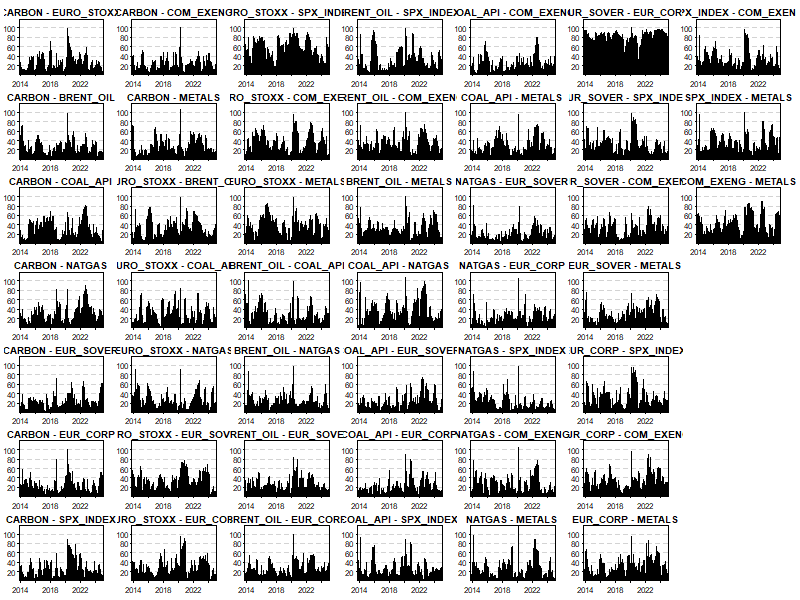
\includegraphics[width = 1.2\linewidth]{25bApdxD-12-180-VolPCI}
    \end{subfigure}
\end{figure}










\subsection{12-period forecast horizon and a rolling window of 200 observations}

\subsubsection{Static Return and Volatility Connectedness Matrix}

  \begin{table}[!ht]
    \caption{Static Return and Volatility Connectedness Matrix (Jan 2013 - Jan 2025)}
      \resizebox{\columnwidth}{!}{
      \begin{tabular}{|l|l|l|l|l|l|l|l|l|l|l|l|}
    \multicolumn{12}{@{}l}{\em(a) Carbon returns connectedness matrix}\\ \hline
        ~ & CARBON & EUROSTOXX & BRENTOIL & COALAPI & NATGAS & EURSOVER & EURCORP & SPXINDEX & COMEXENG & METALS & FROM \\ \hline
        CARBON & 59.98 & 4 & 3.81 & 7.85 & 10.21 & 2.49 & 2.28 & 3.48 & 2.77 & 3.13 & 40.02 \\ \hline
        EUROSTOXX & 3.28 & 49.71 & 5.71 & 3.34 & 3.13 & 3.05 & 3.68 & 19.85 & 5.21 & 3.03 & 50.29 \\ \hline
        BRENTOIL & 3.5 & 6.01 & 57.33 & 5.44 & 3.62 & 2.69 & 2.35 & 7.28 & 8.29 & 3.5 & 42.67 \\ \hline
        COALAPI & 6.34 & 3.78 & 5.8 & 55.96 & 13.77 & 1.86 & 2.05 & 3.84 & 3.96 & 2.64 & 44.04 \\ \hline
        NATGAS & 9.93 & 3.04 & 3.89 & 13.57 & 58.66 & 1.81 & 1.77 & 2.5 & 2.57 & 2.25 & 41.34 \\ \hline
        EURSOVER & 2.04 & 3.01 & 2.69 & 1.68 & 1.69 & 48.28 & 31.89 & 2.3 & 2.06 & 4.36 & 51.72 \\ \hline
        EURCORP & 1.98 & 5.05 & 2.72 & 1.75 & 1.82 & 30.35 & 45.45 & 3.97 & 2.55 & 4.36 & 54.55 \\ \hline
        SPXINDEX & 2.43 & 17.94 & 6.82 & 3.36 & 2.04 & 2.32 & 2.74 & 53.46 & 6.4 & 2.51 & 46.54 \\ \hline
        COMEXENG & 2.49 & 5.09 & 7.45 & 3.49 & 2.41 & 2.17 & 2.38 & 6.6 & 53.02 & 14.9 & 46.98 \\ \hline
        METALS & 2.38 & 3.18 & 3.13 & 2.29 & 2.47 & 4.84 & 5.59 & 2.98 & 16.13 & 57.02 & 42.98 \\ \hline
        DST(TO) & 34.37 & 51.09 & 42.02 & 42.78 & 41.16 & 51.58 & 54.72 & 52.79 & 49.94 & 40.68 & 461.13 \\ \hline
        Inc. Own & 94.35 & 100.8 & 99.35 & 98.74 & 99.82 & 99.86 & 100.17 & 106.25 & 102.96 & 97.69 & cTCI/TCI \\ \hline
        NS (NET) & -5.65 & 0.8 & -0.65 & -1.26 & -0.18 & -0.14 & 0.17 & 6.25 & 2.96 & -2.31 & 51.24/46.11 \\ \hline
    \end{tabular}
    }
    \bigskip
      \resizebox{\columnwidth}{!}{
    \begin{tabular}{|l|l|l|l|l|l|l|l|l|l|l|l|}
    \multicolumn{12}{@{}l}{\em(b) Carbon volatility connectedness matrix}\\ \hline
        ~ & CARBON & EUROSTOXX & BRENTOIL & COALAPI & NATGAS & EURSOVER & EURCORP & SPXINDEX & COMEXENG & METALS & FROM \\ \hline
        CARBON & 51.77 & 4.95 & 4.62 & 7.64 & 7.57 & 4.25 & 4.08 & 5.87 & 4.28 & 4.97 & 48.23 \\ \hline
        EUROSTOXX & 3.95 & 44.7 & 5.26 & 4 & 4.01 & 5.47 & 4.39 & 16.25 & 5.63 & 6.33 & 55.3 \\ \hline
        BRENTOIL & 4.33 & 6.94 & 48.98 & 5.34 & 4.07 & 4.39 & 5.01 & 6.77 & 7.45 & 6.73 & 51.02 \\ \hline
        COALAPI & 5.18 & 6.48 & 4.42 & 54.18 & 8.27 & 4.19 & 3.09 & 5.01 & 3.51 & 5.67 & 45.82 \\ \hline
        NATGAS & 4.87 & 5.04 & 3.94 & 8.7 & 55.58 & 4.08 & 4.28 & 5.31 & 3.85 & 4.35 & 44.42 \\ \hline
        EURSOVER & 2.39 & 6.61 & 3.52 & 2.68 & 2.03 & 43.31 & 24.59 & 5.95 & 4.24 & 4.68 & 56.69 \\ \hline
        EURCORP & 3.04 & 6.01 & 2.75 & 2.55 & 2.71 & 27.87 & 40.08 & 6.26 & 5.14 & 3.58 & 59.92 \\ \hline
        SPXINDEX & 3.75 & 15.2 & 5.1 & 3.55 & 2.01 & 5.11 & 4.18 & 50.28 & 4.96 & 5.87 & 49.72 \\ \hline
        COMEXENG & 2.95 & 8.09 & 4.83 & 4.12 & 4.36 & 5.67 & 5.7 & 7.07 & 47.39 & 9.81 & 52.61 \\ \hline
        METALS & 4.08 & 8.78 & 4.77 & 4.27 & 4.3 & 5.29 & 6.67 & 6.72 & 10.22 & 44.9 & 55.1 \\ \hline
        DST(TO) & 34.53 & 68.1 & 39.22 & 42.85 & 39.32 & 66.32 & 61.99 & 65.21 & 49.29 & 51.99 & 518.82 \\ \hline
        Inc. Own & 86.3 & 112.8 & 88.19 & 97.03 & 94.9 & 109.63 & 102.07 & 115.49 & 96.68 & 96.89 & cTCI/TCI \\ \hline
        NS (NET) & -13.7 & 12.8 & -11.81 & -2.97 & -5.1 & 9.63 & 2.07 & 15.49 & -3.32 & -3.11 & 57.65/51.88 \\ \hline
    \end{tabular}
    }
\end{table}




\subsubsection{Dynamic Return and Volatility Net Directional Connectedness}

\begin{figure}[H]
  \caption{Dynamic Net Directional Connectedness (Jan 2013 – Jan 2025)}
    \centering
      \begin{subfigure}[a]{\textwidth}
        \caption{Dynamic return net directional connectedness}
        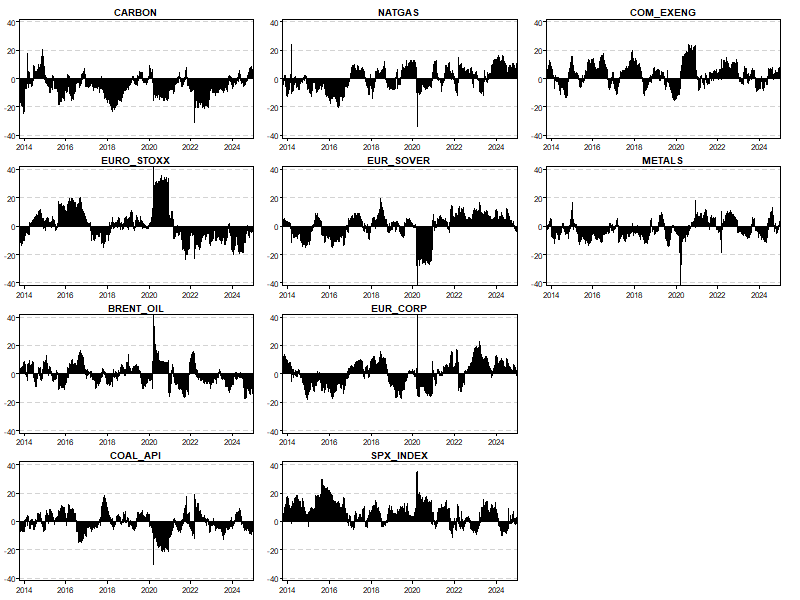
\includegraphics[width = 1.25\linewidth]{26aApdxD-12-200-RetNDC}
      \end{subfigure}
\end{figure}
\begin{figure}[H]
  \ContinuedFloat
  \centering
      \begin{subfigure}[b]{\textwidth}
        \caption{Dynamic volatility net directional connectedness}
        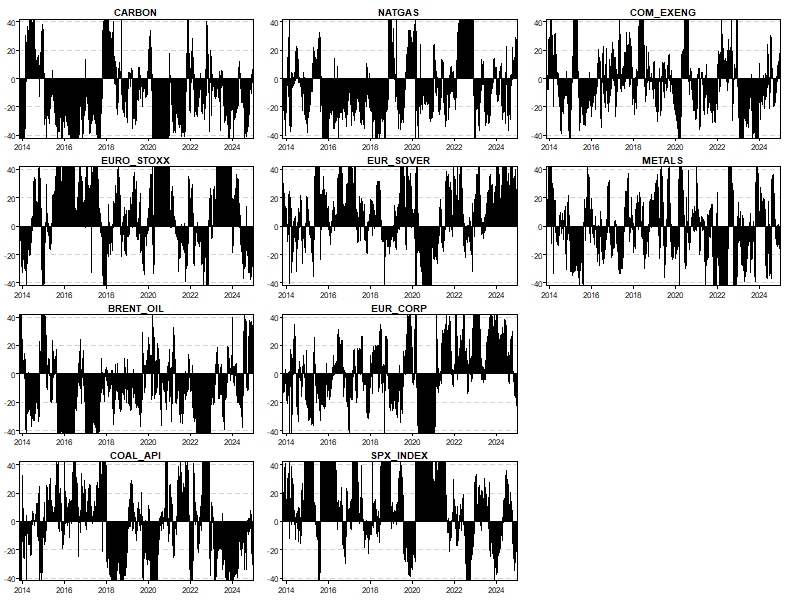
\includegraphics[width = 1.25\linewidth]{26bApdxD-12-200-VolNDC}
      \end{subfigure}
\end{figure}



\subsubsection{Static Return and Volatility Pairwise Directional Connectedness}

\begin{figure}[!ht]
  \caption{Network Representation of Pairwise Connectedness Index (Jan 2013 – Jan 2025)}
  \begin{minipage}{.8\textwidth}
    \subfloat[Static Return PCI network]{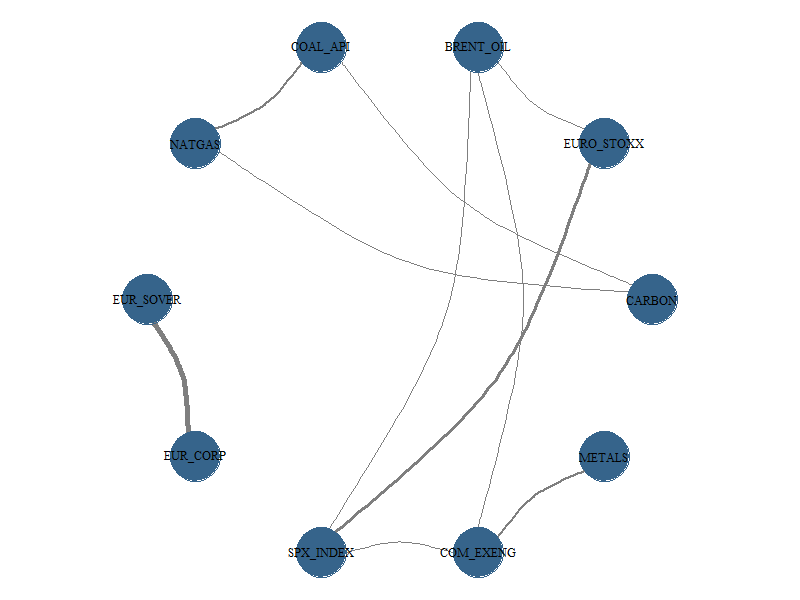
\includegraphics[width = \linewidth]{27aApdxD-12-200-RetNtwrk}}
  \end{minipage}
  \hfill
  \begin{minipage}{.8\textwidth}
    \subfloat[Static Volatility PCI network]{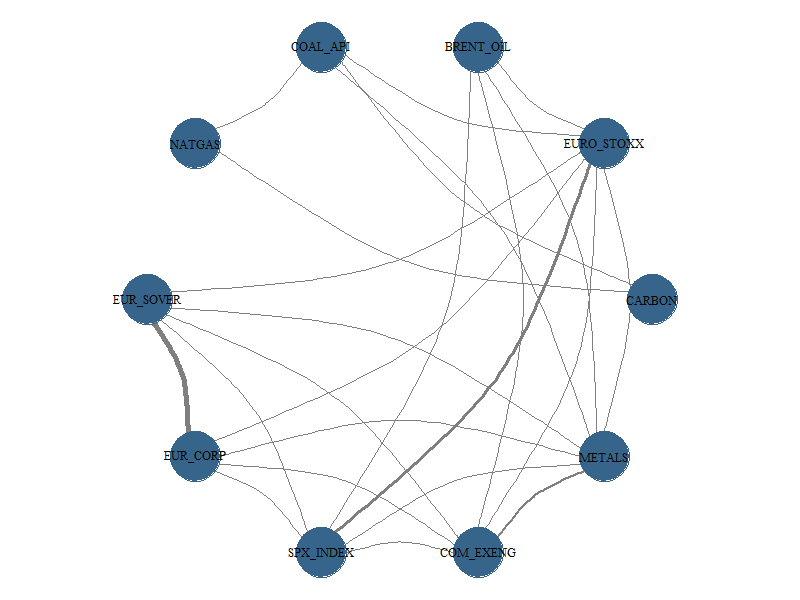
\includegraphics[width = \linewidth]{27bApdxD-12-200-VolNtwrk}}
  \end{minipage}
\end{figure}



\newpage

\subsubsection{Dynamic Return and Volatility Pairwise Directional Connectedness}

\begin{figure}[!ht]
  \caption{Dynamic Return and Volatility Pairwise Connectedness Index (Jan 2013 – Jan 2025)}
  \centering
  \begin{subfigure}[a]{\textwidth}
    \caption{Dynamic return PCI}
    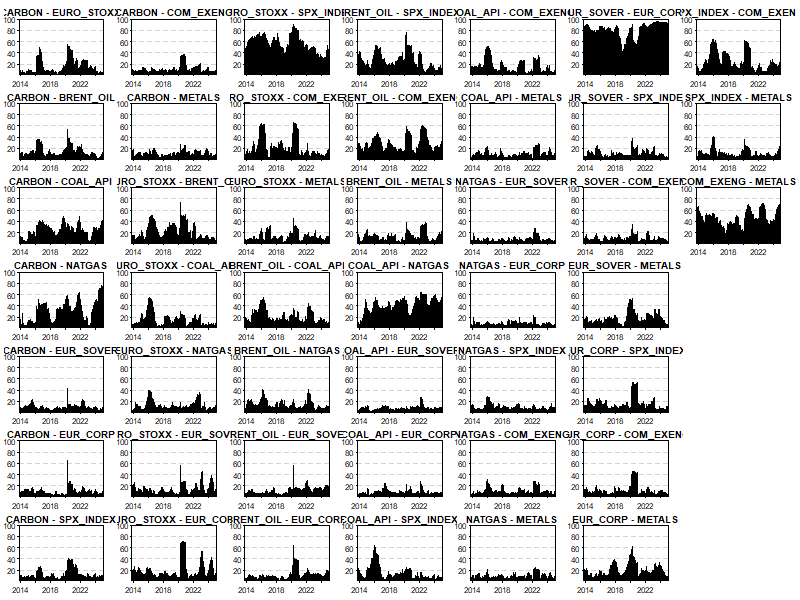
\includegraphics[width = 1.1\linewidth]{28aApdxD-12-200-RetPCI}
  \end{subfigure}
\end{figure}
\begin{figure}[!ht]
  \ContinuedFloat
  \centering
    \begin{subfigure}[b]{\textwidth}\ContinuedFloat
      \caption{Dynamic volatility PCI}
      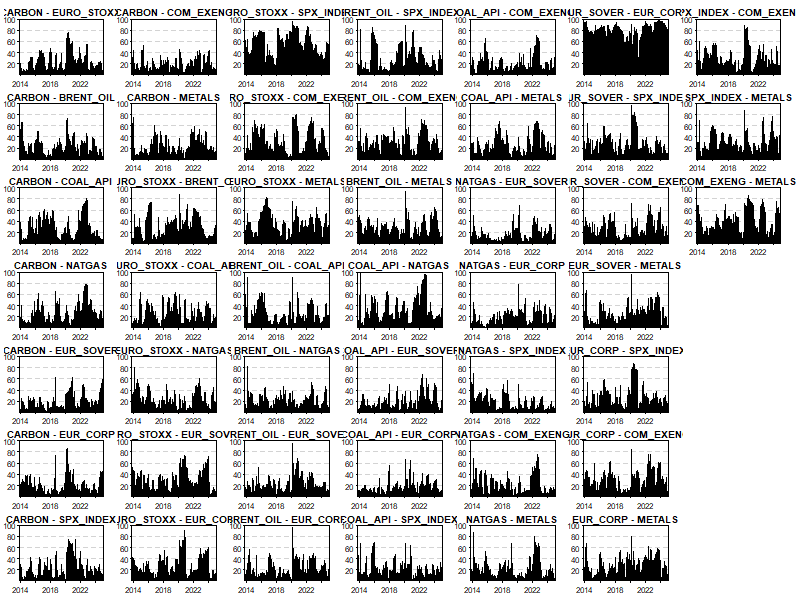
\includegraphics[width = 1.2\linewidth]{28bApdxD-12-200-VolPCI}
    \end{subfigure}
\end{figure}












\subsection{12-period forecast horizon and a rolling window of 220 observations}

\subsubsection{Static Return and Volatility Connectedness Matrix}

  \begin{table}[!ht]
    \caption{Static Return and Volatility Connectedness Matrix (Jan 2013 - Jan 2025)}
      \resizebox{\columnwidth}{!}{
      \begin{tabular}{|l|l|l|l|l|l|l|l|l|l|l|l|}
    \multicolumn{12}{@{}l}{\em(a) Carbon returns connectedness matrix}\\ \hline
        ~ & CARBON & EUROSTOXX & BRENTOIL & COALAPI & NATGAS & EURSOVER & EURCORP & SPXINDEX & COMEXENG & METALS & FROM \\ \hline
        CARBON & 61.29 & 3.94 & 3.67 & 7.78 & 10.07 & 2.3 & 2.13 & 3.29 & 2.61 & 2.93 & 38.71 \\ \hline
        EUROSTOXX & 3.18 & 50.75 & 5.67 & 3.23 & 2.95 & 2.75 & 3.44 & 20.11 & 5.14 & 2.78 & 49.25 \\ \hline
        BRENTOIL & 3.31 & 5.92 & 58.37 & 5.39 & 3.49 & 2.52 & 2.23 & 7.2 & 8.31 & 3.26 & 41.63 \\ \hline
        COALAPI & 6.22 & 3.66 & 5.74 & 56.99 & 13.87 & 1.72 & 1.89 & 3.7 & 3.83 & 2.39 & 43.01 \\ \hline
        NATGAS & 9.79 & 2.87 & 3.75 & 13.75 & 59.92 & 1.63 & 1.61 & 2.24 & 2.38 & 2.06 & 40.08 \\ \hline
        EURSOVER & 1.87 & 2.8 & 2.48 & 1.5 & 1.48 & 49.27 & 32.33 & 2.16 & 1.85 & 4.26 & 50.73 \\ \hline
        EURCORP & 1.84 & 5 & 2.61 & 1.57 & 1.62 & 30.67 & 46.12 & 3.92 & 2.43 & 4.23 & 53.88 \\ \hline
        SPXINDEX & 2.26 & 18.11 & 6.71 & 3.22 & 1.81 & 2.14 & 2.59 & 54.44 & 6.44 & 2.29 & 45.56 \\ \hline
        COMEXENG & 2.33 & 5.03 & 7.43 & 3.35 & 2.18 & 1.97 & 2.22 & 6.63 & 53.89 & 14.98 & 46.11 \\ \hline
        METALS & 2.22 & 2.93 & 2.91 & 2.08 & 2.25 & 4.77 & 5.51 & 2.77 & 16.29 & 58.28 & 41.72 \\ \hline
        DST(TO) & 33.01 & 50.26 & 40.96 & 41.87 & 39.71 & 50.46 & 53.95 & 52 & 49.28 & 39.18 & 450.7 \\ \hline
        Inc. Own & 94.3 & 101.01 & 99.33 & 98.86 & 99.62 & 99.73 & 100.06 & 106.44 & 103.17 & 97.47 & cTCI/TCI \\ \hline
        NS (NET) & -5.7 & 1.01 & -0.67 & -1.14 & -0.38 & -0.27 & 0.06 & 6.44 & 3.17 & -2.53 & 50.08/45.07 \\ \hline
    \end{tabular}
    }
    \bigskip
      \resizebox{\columnwidth}{!}{
    \begin{tabular}{|l|l|l|l|l|l|l|l|l|l|l|l|}
    \multicolumn{12}{@{}l}{\em(b) Carbon volatility connectedness matrix}\\ \hline
        ~ & CARBON & EUROSTOXX & BRENTOIL & COALAPI & NATGAS & EURSOVER & EURCORP & SPXINDEX & COMEXENG & METALS & FROM \\ \hline
        CARBON & 53.98 & 4.97 & 4.32 & 7.64 & 7.18 & 3.84 & 3.72 & 5.49 & 4.29 & 4.56 & 46.02 \\ \hline
        EUROSTOXX & 3.55 & 46.21 & 4.99 & 3.61 & 3.61 & 5.32 & 4.27 & 16.81 & 5.63 & 6.01 & 53.79 \\ \hline
        BRENTOIL & 3.82 & 6.9 & 51.01 & 5.18 & 3.86 & 3.98 & 4.53 & 6.63 & 7.62 & 6.47 & 48.99 \\ \hline
        COALAPI & 5.06 & 5.98 & 3.68 & 57.01 & 7.87 & 3.96 & 2.92 & 4.6 & 3.39 & 5.53 & 42.99 \\ \hline
        NATGAS & 4.63 & 4.71 & 3.52 & 8.47 & 58.3 & 3.77 & 4.15 & 4.94 & 3.53 & 3.99 & 41.7 \\ \hline
        EURSOVER & 2.06 & 6.39 & 3.31 & 2.32 & 1.72 & 44.95 & 25.12 & 5.85 & 3.77 & 4.53 & 55.05 \\ \hline
        EURCORP & 2.67 & 6.01 & 2.68 & 2.1 & 2.2 & 28.56 & 41.62 & 6.19 & 4.53 & 3.42 & 58.38 \\ \hline
        SPXINDEX & 3.46 & 15.35 & 4.67 & 3.27 & 1.77 & 4.68 & 3.85 & 52.71 & 4.66 & 5.58 & 47.29 \\ \hline
        COMEXENG & 2.45 & 8.05 & 4.81 & 3.83 & 3.94 & 5.14 & 5.21 & 6.79 & 49.88 & 9.9 & 50.12 \\ \hline
        METALS & 3.87 & 8.67 & 4.35 & 4 & 3.91 & 5.1 & 6.19 & 6.11 & 10.51 & 47.28 & 52.72 \\ \hline
        DST(TO) & 31.56 & 67.03 & 36.35 & 40.42 & 36.07 & 64.35 & 59.96 & 63.39 & 47.93 & 49.97 & 497.04 \\ \hline
        Inc. Own & 85.54 & 113.25 & 87.36 & 97.43 & 94.38 & 109.3 & 101.59 & 116.09 & 97.81 & 97.25 & cTCI/TCI \\ \hline
        NS (NET) & -14.46 & 13.25 & -12.64 & -2.57 & -5.62 & 9.3 & 1.59 & 16.09 & -2.19 & -2.75 & 55.23/49.70 \\ \hline
    \end{tabular}
    }
\end{table}




\subsubsection{Dynamic Return and Volatility Net Directional Connectedness}

\begin{figure}[H]
  \caption{Dynamic Net Directional Connectedness (Jan 2013 – Jan 2025)}
    \centering
      \begin{subfigure}[a]{\textwidth}
        \caption{Dynamic return net directional connectedness}
        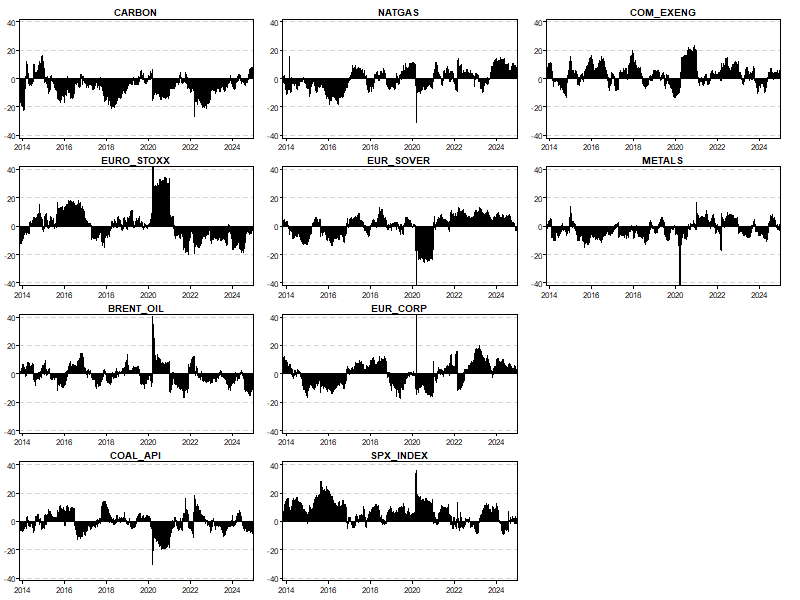
\includegraphics[width = 1.25\linewidth]{29aApdxD-12-220-RetNDC}
      \end{subfigure}
\end{figure}
\begin{figure}[H]
  \ContinuedFloat
  \centering
      \begin{subfigure}[b]{\textwidth}
        \caption{Dynamic volatility net directional connectedness}
        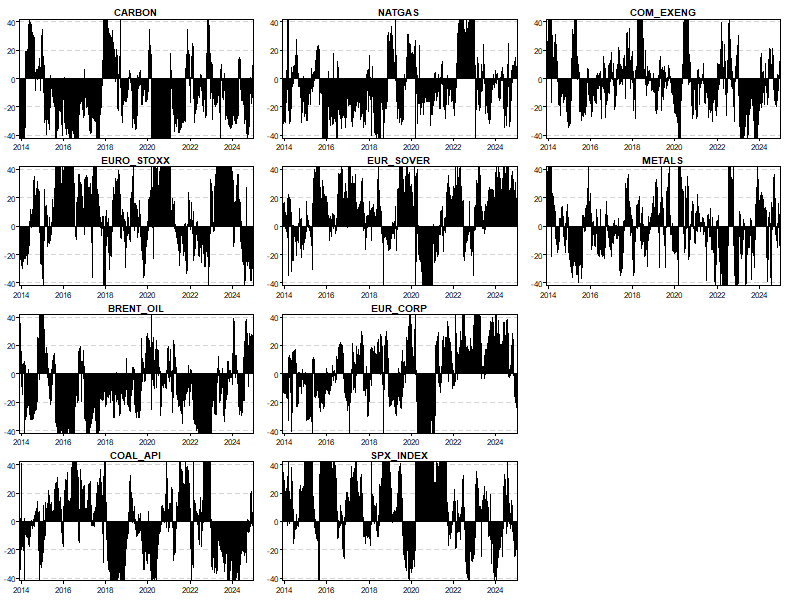
\includegraphics[width = 1.25\linewidth]{29bApdxD-12-220-VolNDC}
      \end{subfigure}
\end{figure}



\subsubsection{Static Return and Volatility Pairwise Directional Connectedness}

\begin{figure}[!ht]
  \caption{Network Representation of Pairwise Connectedness Index (Jan 2013 – Jan 2025)}
  \begin{minipage}{.8\textwidth}
    \subfloat[Static Return PCI network]{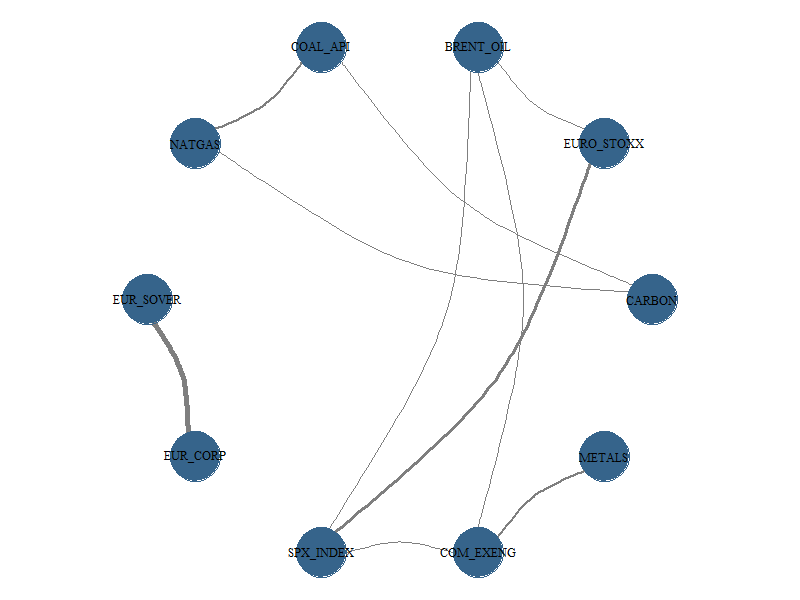
\includegraphics[width = \linewidth]{30aApdxD-12-220-RetNtwrk}}
  \end{minipage}
  \hfill
  \begin{minipage}{.8\textwidth}
    \subfloat[Static Volatility PCI network]{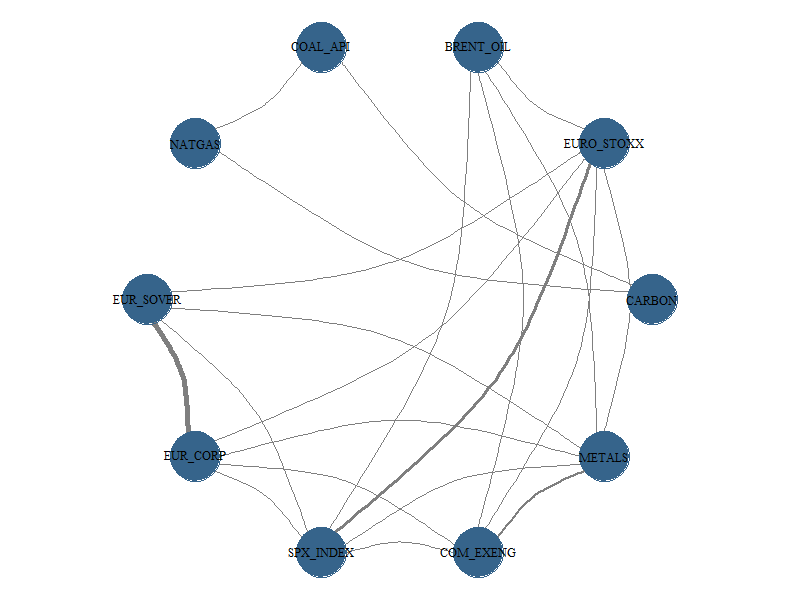
\includegraphics[width = \linewidth]{30bApdxD-12-220-VolNtwrk}}
  \end{minipage}
\end{figure}



\newpage

\subsubsection{Dynamic Return and Volatility Pairwise Directional Connectedness}

\begin{figure}[!ht]
  \caption{Dynamic Return and Volatility Pairwise Connectedness Index (Jan 2013 – Jan 2025)}
  \centering
  \begin{subfigure}[a]{\textwidth}
    \caption{Dynamic return PCI}
    \includegraphics[width = 1.1\linewidth]{31aApdxD-12-220-RetPCI}
  \end{subfigure}
\end{figure}
\begin{figure}[!ht]
  \ContinuedFloat
  \centering
    \begin{subfigure}[b]{\textwidth}\ContinuedFloat
      \caption{Dynamic volatility PCI}
      \includegraphics[width = 1.2\linewidth]{31bApdxD-12-220-VolPCI}
    \end{subfigure}
\end{figure}










\end{landscape}

\newpage

\bibliography{EUAbibliography.bib}


\end{document}
